\documentclass{rapport}
\usepackage[backend=bibtex]{biblatex}
\addbibresource{referencias.bib}
\usepackage{lipsum}
\usepackage{gensymb}
\usepackage{float}
\usepackage{graphicx} % Required for inserting images
\usepackage{array}
\usepackage{adjustbox}
\usepackage[utf8]{inputenc} 
\usepackage[T1]{fontenc}     
\usepackage[spanish]{babel}  
\usepackage{tabularx}
\usepackage{listings}
\usepackage{xcolor}
\usepackage{courier} % Para fuente tipo consola

%New colors defined below
\definecolor{codecyan}{rgb}{0.0, 0.7, 0.9}
\definecolor{codegray}{rgb}{0.9,0.9,0.9}
\definecolor{codepurple}{rgb}{0.58,0,0.82}
\definecolor{backcolour}{rgb}{0.95,0.95,0.92}

% Colores personalizados
\usepackage{xcolor}
\definecolor{codegray}{rgb}{1,1,1}
\definecolor{backcolour}{rgb}{0.95,0.95,0.95}
\definecolor{codecyan}{rgb}{0.0,0.6,0.6}
\definecolor{codepurple}{rgb}{0.58,0,0.82}

% Estilo para código en R
\lstdefinestyle{rstyle}{
  language=R,
  backgroundcolor=\color{backcolour},  % Color de fondo claro para mejor legibilidad
  basicstyle=\ttfamily\small,
  keywordstyle=\color{codecyan}\bfseries,
  commentstyle=\color{orange}\itshape,
  stringstyle=\color{codepurple},
  frame=single,
  breaklines=true,
  numbers=left,
  numberstyle=\tiny\color{codegray},
  showstringspaces=false
}

\begin{document}

%----------- Información del reporte ---------

\logo{logos/logo.png}
\uni{\textbf{Universidad de Cartagena}}
\ttitle{Análisis del IMC en Función del Programa Académico y la Edad en Estudiantes de la Universidad de Cartagena} % Título del documento
\subject{Diseño de Experimentos} % Nombre de la materia
\topic{Diseño de Experimentos} % Tema del trabajo

\professor{Luz Elena Vargas Ortiz} % Información del profesor

\students{Sharon Nicole Acosta Caraballo\\
          María José Ibarra Ariña}  % Información de los estudiantes

%----------- Inicio del documento -------------------
        
\buildmargins % Mostrar márgenes
\buildcover % Crear portada
\tableofcontents % Generar tabla de contenido
\newpage
%------------ Cuerpo del reporte ----------------

\section*{Resumen}
Este estudio analiza las posibles diferencias en el Índice de Masa Corporal (IMC) entre estudiantes de los programas de Matemáticas, Biología y Química en la Universidad de Cartagena, considerando además el género y el grupo etario (17–19, 20–22 y 23–31 años). La investigación se realizó mediante la recolección de datos de 60 estudiantes, distribuidos equitativamente en los diferentes programas, géneros. Para analizar los efectos de estas variables sobre el IMC, se aplicó un análisis de varianza factorial (ANOVA) de tres vías, permitiendo identificar efectos principales e interacciones significativas. Los resultados muestran que tanto el programa académico como el género y el grupo etario influyen en el IMC, con interacciones que sugieren que estos factores no actúan de manera independiente. Las conclusiones indican la importancia de considerar múltiples variables al evaluar el estado nutricional en la población universitaria, y abren la posibilidad de desarrollar estrategias específicas para mejorar la salud de los estudiantes.

\vspace{0.5cm}

\textbf{Palabras clave:} IMC, ANOVA, estudiantes universitarios, grupo etario, género, programa académico. 



\newpage

\section*{Introducción}

El estado nutricional de los estudiantes universitarios es un tema de interés debido a su impacto en la salud, el rendimiento académico y el bienestar general. El Índice de Masa Corporal (IMC) es una de las herramientas más utilizadas para evaluar el peso en relación con la estatura y detectar posibles problemas de sobrepeso o desnutrición. 

\vspace{0.5cm}

Diversos estudios han señalado que factores como el programa académico, el género y la edad pueden influir en el IMC, pero aún se necesita investigar cómo estas variables interactúan en poblaciones específicas, como la de estudiantes de la Universidad de Cartagena. Por ejemplo, \textcite{nieto2021habitos} encontraron una tendencia hacia el sobrepeso y la obesidad en estudiantes universitarios de Cultura Física en Barranquilla, subrayando la importancia de monitorear el IMC en contextos académicos diversos.

\vspace{0.5cm}

Este estudio busca analizar las diferencias en el IMC entre estudiantes de los programas de Matemáticas, Biología y Química, considerando además el género y los grupos etarios, con el fin de aportar información relevante para el diseño de estrategias de promoción de la salud en la comunidad universitaria.


\newpage

\section{Metodología}

Para este estudio se recolectaron datos de estudiantes de la Universidad de Cartagena, con el propósito de analizar si existen diferencias en el índice de masa corporal (IMC) según el programa académico, el género y la edad. El IMC se calculó a partir de los datos de peso y estatura proporcionados voluntariamente por los propios estudiantes. Además, se registró la edad y el género de cada participante.



\section{Población y muestra}

La población objetivo del estudio estuvo conformada por estudiantes activos de los programas de Matemáticas, Biología y Química de la Universidad de Cartagena.

Se utilizó un muestreo por conveniencia, seleccionando un total de \textbf{60 estudiantes}, distribuidos equitativamente entre los tres programas académicos, con 20 estudiantes por programa. A su vez, en cada programa se incluyeron 10 estudiantes de género femenino y 10 de género masculino, garantizando el equilibrio entre los niveles del factor género.

\vspace{0.5cm}

Posteriormente, se categorizó la variable edad en tres grupos: \textbf{17--19 años}, \textbf{20--22 años} y \textbf{23--31 años}, lo que permitió estructurar un diseño factorial de tipo $3 \times 2 \times 3$, correspondiente a \textbf{tres programas}, \textbf{dos géneros} y \textbf{tres grupos de edad}.

\vspace{0.5cm}

Esta distribución dio lugar a un análisis multifactorial con \textbf{18 combinaciones posibles}, permitiendo examinar tanto los efectos principales de cada factor como las interacciones entre ellos respecto al índice de masa corporal (IMC).


\section{Variables del diseño experimental}

En este estudio, se identificaron las siguientes variables:

\begin{itemize}
    \item \textbf{Variable de respuesta (dependiente):}
    \begin{itemize}
        \item \textbf{Índice de Masa Corporal (IMC)}: Variable cuantitativa continua. Se calcula a partir del peso y la estatura de cada estudiante mediante la fórmula: 
        \[
        \text{IMC} = \frac{\text{Peso (kg)}}{[\text{Estatura (m)}]^2}
        \]
        Esta variable es la respuesta del estudio, ya que se analiza su comportamiento frente a las diferentes combinaciones de factores.
    \end{itemize}
    
    \item \textbf{Variables independientes (factores):}
    \begin{itemize}
        \item \textbf{Programa académico}: Variable cualitativa nominal con tres niveles: Matemáticas, Biología y Química.
        \item \textbf{Género}: Variable cualitativa nominal con dos niveles: Femenino y Masculino.
        \item \textbf{Grupo de edad}: Variable cualitativa ordinal categorizada en tres niveles: 17--19 años, 20--22 años y 23--31 años.
    \end{itemize}
    
    \item \textbf{Variables auxiliares (usadas para calcular el IMC):}
    \begin{itemize}
        \item \textbf{Peso}: Variable cuantitativa continua, expresada en kilogramos (kg).
        \item \textbf{Estatura}: Variable cuantitativa continua, expresada en metros (m).
        \item \textbf{Edad}: Variable cuantitativa discreta (en años), utilizada para clasificar a los participantes en los tres grupos etarios definidos.
    \end{itemize}
\end{itemize}


\section{Diseño experimental}

El diseño implementado en este estudio es un \textbf{diseño factorial completo $3 \times 2 \times 3$}, donde se analizaron de forma simultánea tres factores: \textit{Programa académico} (con 3 niveles), \textit{Género} (con 2 niveles) y \textit{Grupo de edad} (con 3 niveles). Este diseño permite estudiar no solo los efectos principales de cada factor sobre el índice de masa corporal (IMC), sino también las posibles interacciones entre ellos.

\vspace{0.5cm}

Para el análisis estadístico, se utilizaron herramientas del lenguaje de programación R. En primera instancia, los datos fueron cargados desde un archivo en Excel denominado 'CienciasExactasIMC', la cual fue importada junto con las librerías necesarias para el análisis a realizar

\begin{lstlisting}[style=rstyle]
attach(CienciasExactasIMC)
library(modeest)
library(moments)
library(readxl)
library(dplyr)
library(ggplot2)
library(car)
library(agricolae)
library(PMCMRplus)
\end{lstlisting}

 Luego, se creó una nueva variable categórica denominada \texttt{GrupoEdad}, la cual clasifica la edad de los participantes en tres grupos: 17--19, 20--22 y 23--31 años, de acuerdo con el resumen de la variable original \texttt{e} (Edad):

\begin{lstlisting}[style=rstyle]
summary(CienciasExactasIMC$e)

CienciasExactasIMC$GrupoEdad <- cut(CienciasExactasIMC$e,
                                    breaks = c(16, 19, 22, 32),
                                    labels = c("17-19", "20-22", "23-31"),
                                    right = TRUE)

table(CienciasExactasIMC$GrupoEdad)
\end{lstlisting}

A partir de estas tres variables categóricas: \texttt{Programa}, \texttt{Género} y \texttt{GrupoEdad}, se ajustó un modelo lineal mediante un análisis de varianza (ANOVA) factorial:

\begin{lstlisting}[style=rstyle]
Modelo <- aov(IMC ~ Programa * Genero * GrupoEdad, 
          data = CienciasExactasIMC)
\end{lstlisting}

Este modelo incluye:

\begin{itemize}
    \item Los efectos principales de cada factor
    \item Todas las interacciones de segundo orden
    \item La interacción de tercer orden entre los tres factores
\end{itemize}

Posteriormente, se extrajeron los residuos del modelo para evaluar el cumplimiento de los supuestos asociados al ANOVA, como la normalidad, independencia y homogeneidad de varianzas:

\begin{lstlisting}[style=rstyle]
residuos <- residuals(Modelo)
\end{lstlisting}

\subsection{Prueba de los supuestos del modelo}

\subsubsection{Normalidad} 
Para verificar el supuesto de normalidad, realizamos la prueba de Shapiro-Wilk. Utilizando el siguiente comando:

\begin{lstlisting}[style=rstyle]
shapiro.test(Modelo$residuals)
\end{lstlisting}

Obteniendo los siguientes resultados : 

\begin{verbatim}
    Shapiro-Wilk normality test

    data:  Modelo$residuals
    W = 0.97912, p-value = 0.3925
\end{verbatim}

La \textbf{prueba de Shapiro-Wilk} es un test estadístico utilizado para evaluar si una muestra proviene de una \textbf{distribución normal}. Es especialmente útil para tamaños de muestra pequeños o moderados.

La prueba considera las siguientes hipótesis:
\begin{itemize}
    \item Hipótesis nula (\(H_0\)): los datos provienen de una distribución normal.
    \item Hipótesis alternativa (\(H_1\)): los datos no provienen de una distribución normal.
\end{itemize}

El estadístico de prueba es \(W\), que toma valores entre 0 y 1. Cuanto más cercano esté \(W\) a 1, mayor evidencia hay a favor de la normalidad. Sin embargo, la interpretación formal se basa en el \textit{p-valor}.\cite{montgomery2019diseno}\\

En este caso, se obtuvo \(W = 0.97912\) y un \textit{p-valor} de 0.3925. Como este valor es mayor que el nivel de significancia usual (\(\alpha = 0.05\)), \textbf{no se rechaza la hipótesis nula}. \\

Por lo tanto, se concluye que \textbf{no hay evidencia suficiente para afirmar que los residuos no siguen una distribución normal}. Es decir, los residuos pueden considerarse \textbf{normalmente distribuidos}, cumpliendo así con uno de los supuestos fundamentales del modelo lineal.

\vspace{0.5cm}

Visualmente se puede afirmar tal conclusión con el siguiente gráfico:

\begin{figure}[H]
    \centering
    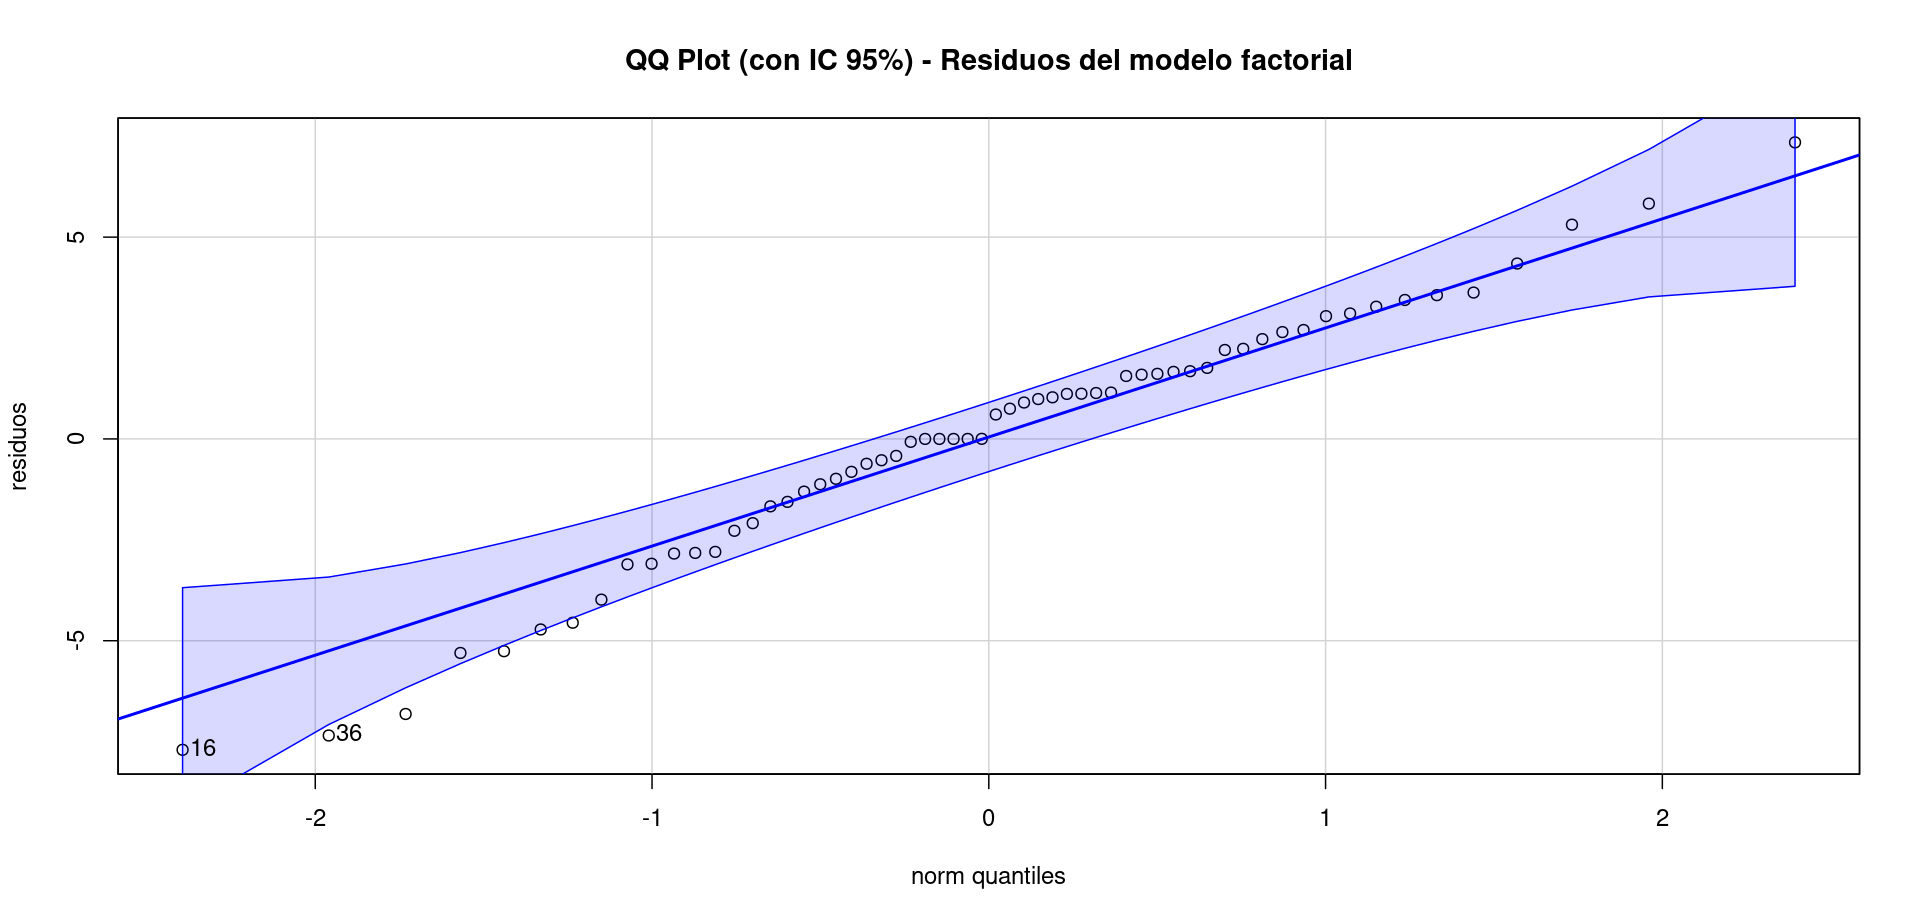
\includegraphics[width=1\textwidth]{normalidad_IMC.png}
    \caption{QQ Plot (con IC 95\%) de los residuos del modelo factorial. La línea azul representa la distribución normal teórica. Los puntos deben seguir esta línea si los residuos se distribuyen normalmente.}
    \label{fig:qqplot}
\end{figure}

El gráfico QQ (Quantile-Quantile) compara los cuantiles observados de los residuos del modelo factorial con los cuantiles esperados bajo una distribución normal.

En el gráfico:
\begin{itemize}
    \item Los puntos representan los residuos ordenados del modelo.
    \item La línea azul indica la línea de referencia donde se ubicarían los puntos si siguieran una distribución normal perfecta.
    \item La banda azul representa un intervalo de confianza del 95\%.
\end{itemize}

Se observa que:
\begin{itemize}
    \item La mayoría de los puntos se encuentran alineados con la línea de referencia y dentro de la banda de confianza.
    \item Sólo unos pocos puntos en las colas presentan una leve desviación, lo cual es esperable en datos reales.
    \item No se detectan patrones sistemáticos de curvatura (como forma de "S"), lo que indicaría asimetría o problemas de curtosis.
\end{itemize}

En conclusión el gráfico QQ no muestra desviaciones importantes respecto a la normalidad, por lo tanto, se refuerza la conclusión obtenida con la prueba de Shapiro-Wilk. Podemos asumir que los residuos del modelo factorial siguen una distribución aproximadamente normal.

\subsubsection{Independencia}
Para verificar el supuesto de independencia, realizamos la prueba de Prueba Durbin-Watson (DW).  Empleando el siguiente comando : 

\begin{lstlisting}[style=rstyle]
dwtest(Modelo)
\end{lstlisting}

Obteniendo los siguientes resultados : 
\begin{verbatim}
    Durbin-Watson test

    data:  Modelo
    DW = 2.2983, p-value = 0.868
    alternative hypothesis: true autocorrelation is greater than 0
\end{verbatim}

La \textbf{prueba de Durbin-Watson} se utiliza para detectar la presencia de \textbf{autocorrelación de primer orden} en los residuos de un modelo de regresión. Este supuesto es importante, ya que la autocorrelación viola uno de los supuestos clave del modelo lineal clásico: la independencia de los errores.\\

Las hipótesis de la prueba son:
\begin{itemize}
    \item \( H_0 \): No hay autocorrelación en los residuos (los errores son independientes).
    \item \( H_1 \): Existe autocorrelación positiva de primer orden.
\end{itemize}

El \textbf{estadístico de Durbin-Watson}, denotado como \( DW \), toma valores entre 0 y 4:
\begin{itemize}
    \item \( DW \approx 2 \): No hay autocorrelación.
    \item \( DW < 2 \): Indica autocorrelación positiva.
    \item \( DW > 2 \): Indica autocorrelación negativa.
\end{itemize}

En este caso, el resultado fue:
\begin{itemize}
    \item \( DW = 2.2983 \), lo cual está cercano a 2 y sugiere independencia de los errores.
    \item El \textit{p-valor} es 0.868, valor considerablemente mayor que el nivel de significancia \(\alpha = 0.05\), por lo que \textbf{no se rechaza la hipótesis nula}.
\end{itemize}\cite{cerda2002diseno}

En conclusión no hay evidencia estadística de autocorrelación en los residuos. Por lo tanto, se puede asumir que los errores del modelo son independientes.

\begin{figure}[H]
    \centering
    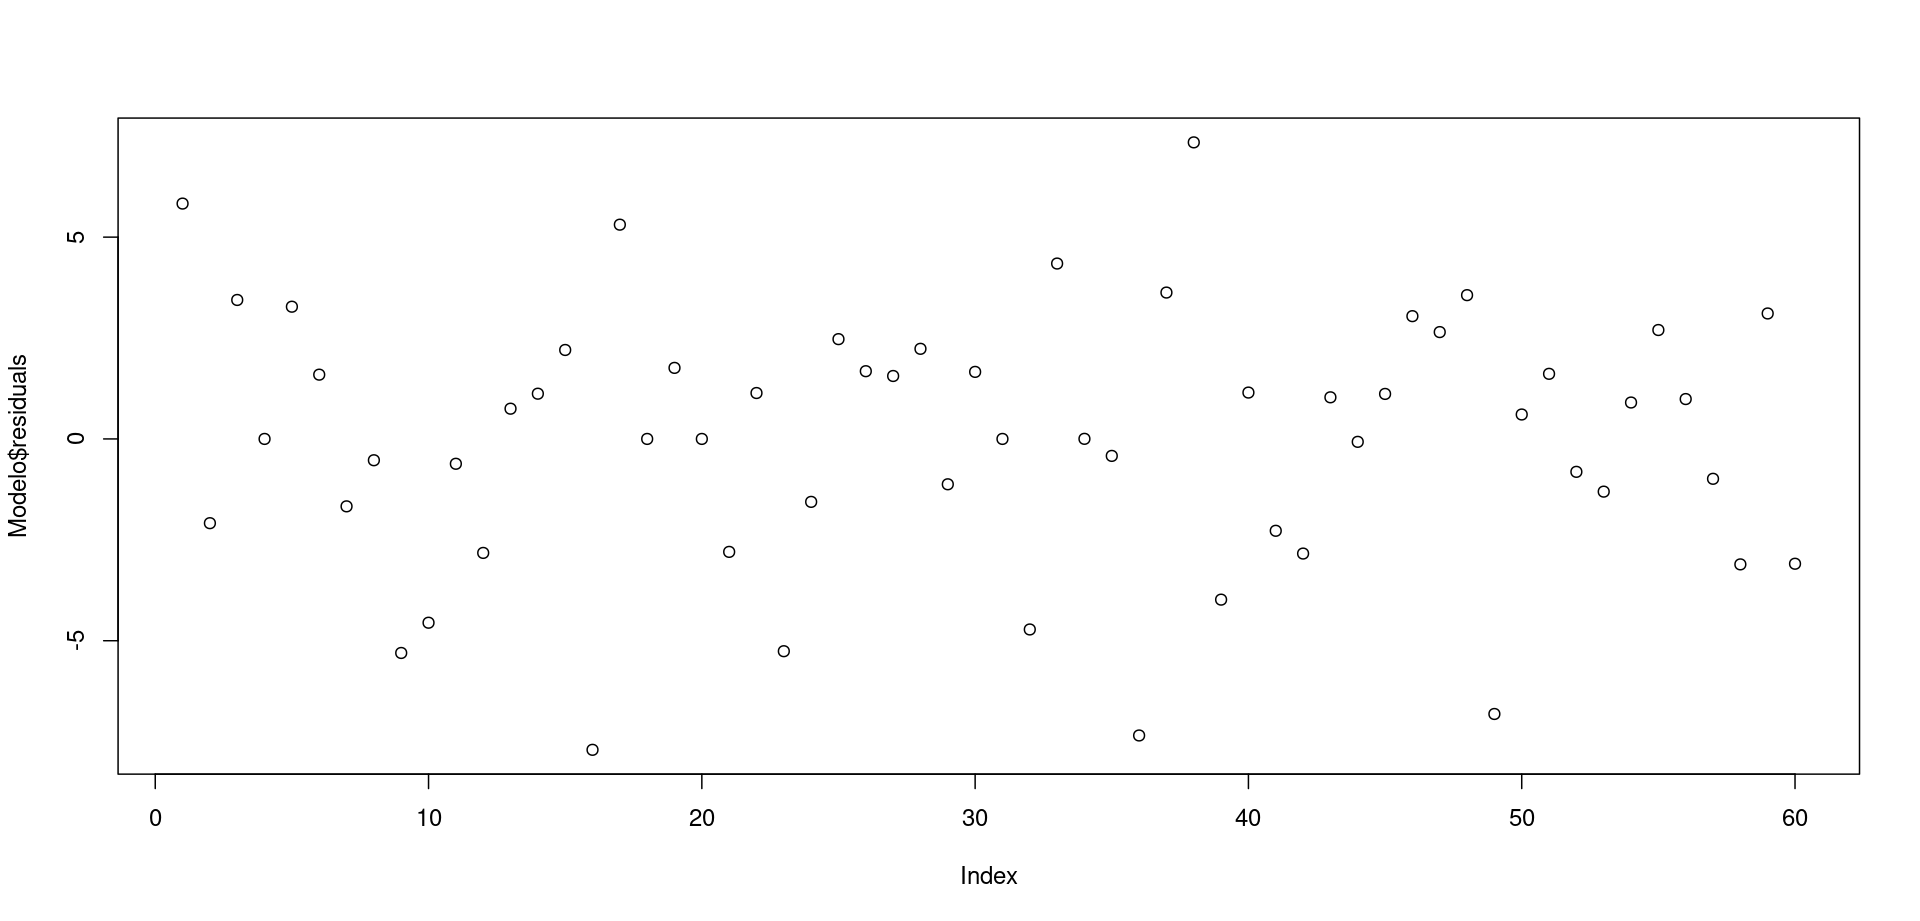
\includegraphics[width=0.95\textwidth]{grafico_dispresion_independencia.png}
    \caption{Gráfico de dispersión de los residuos del modelo factorial. Se observa la distribución de los residuos respecto a su índice, útil para verificar supuestos como homocedasticidad e independencia.}
    \label{fig:residuos-index}
\end{figure}

Este gráfico representa los residuos del modelo frente al índice de observación. Es útil para verificar el supuesto de \textbf{independencia de los errores}.

\begin{itemize}
    \item En el eje horizontal se muestra el índice de cada observación.
    \item En el eje vertical se representan los residuos del modelo.
\end{itemize}

\textbf{Criterios de evaluación:}
\begin{itemize}
    \item Si los errores son independientes, los puntos deben distribuirse de forma \textbf{aleatoria} alrededor de la línea horizontal \( y = 0 \).
    \item No deben observarse patrones sistemáticos, agrupamientos, ni formas cíclicas.
\end{itemize}

\textbf{Observación del gráfico:}
\begin{itemize}
    \item Los residuos parecen dispersarse de forma aleatoria.
    \item No se detectan estructuras cíclicas, tendencias u oscilaciones.
    \item La variabilidad de los residuos no muestra cambios notorios a lo largo del índice.
\end{itemize}

En conclusión el gráfico no muestra evidencia visual de autocorrelación en los residuos. Esto respalda la conclusión obtenida a partir de la prueba de Durbin-Watson: los errores del modelo pueden considerarse \textbf{independientes}.

\subsubsection{Homogeneidad de varianzas}
Para verificar el supuesto de homogeneidad de varianzas, realizamos la prueba de Levence. Con lo cual, empleamos el siguiente comando

\begin{lstlisting}[style=rstyle]
leveneTest(IMC ~ Programa * Genero * GrupoEdad, 
data = CienciasExactasIMC)
\end{lstlisting}

Obteniendo los siguientes resultados:

\begin{verbatim}
    Levene's Test for Homogeneity of Variance (center = median)
      Df F value Pr(>F)
group 16  1.2476 0.2738
      43 
\end{verbatim}

La \textbf{prueba de Levene} se utiliza para verificar el supuesto de \textbf{homogeneidad de varianzas} entre grupos. Este supuesto es fundamental en el análisis de la varianza (ANOVA) y en modelos lineales, ya que muchas pruebas estadísticas asumen que las varianzas de los errores son iguales en todos los niveles de los factores.\\

En esta prueba se evalúan las siguientes hipótesis:

\begin{itemize}
    \item \( H_0 \): Las varianzas de los grupos son iguales (homocedasticidad).
    \item \( H_1 \): Al menos una de las varianzas difiere de las demás (heterocedasticidad).
\end{itemize}

El test fue aplicado sobre los grupos definidos por la interacción de \texttt{Programa}, \texttt{Género} y \texttt{GrupoEdad}, utilizando la mediana como centro.

Se obtuvieron los siguientes resultados:
\begin{itemize}
    \item Grados de libertad: \( \text{Df}_{grupo} = 16 \), \( \text{Df}_{residuos} = 43 \).
    \item Estadístico \( F = 1.2476 \).
    \item \textit{p-valor} = 0.2738.
\end{itemize}

Dado que el \textit{p-valor} = 0.2738. es mayor que el nivel de significancia habitual (\( \alpha = 0.05 \)), \textbf{no se rechaza la hipótesis nula}. Esto indica que no existen diferencias significativas entre las varianzas de los grupos definidos por la combinación de factores.\\

En conclusión se puede asumir \textbf{homogeneidad de varianzas} en los datos, cumpliéndose así uno de los supuestos clave del modelo.

 \vspace{0.5cm}
Visualmente se puede afirmar tal conclusión con el siguiente gráfico:

\begin{figure}[H]
    \centering
    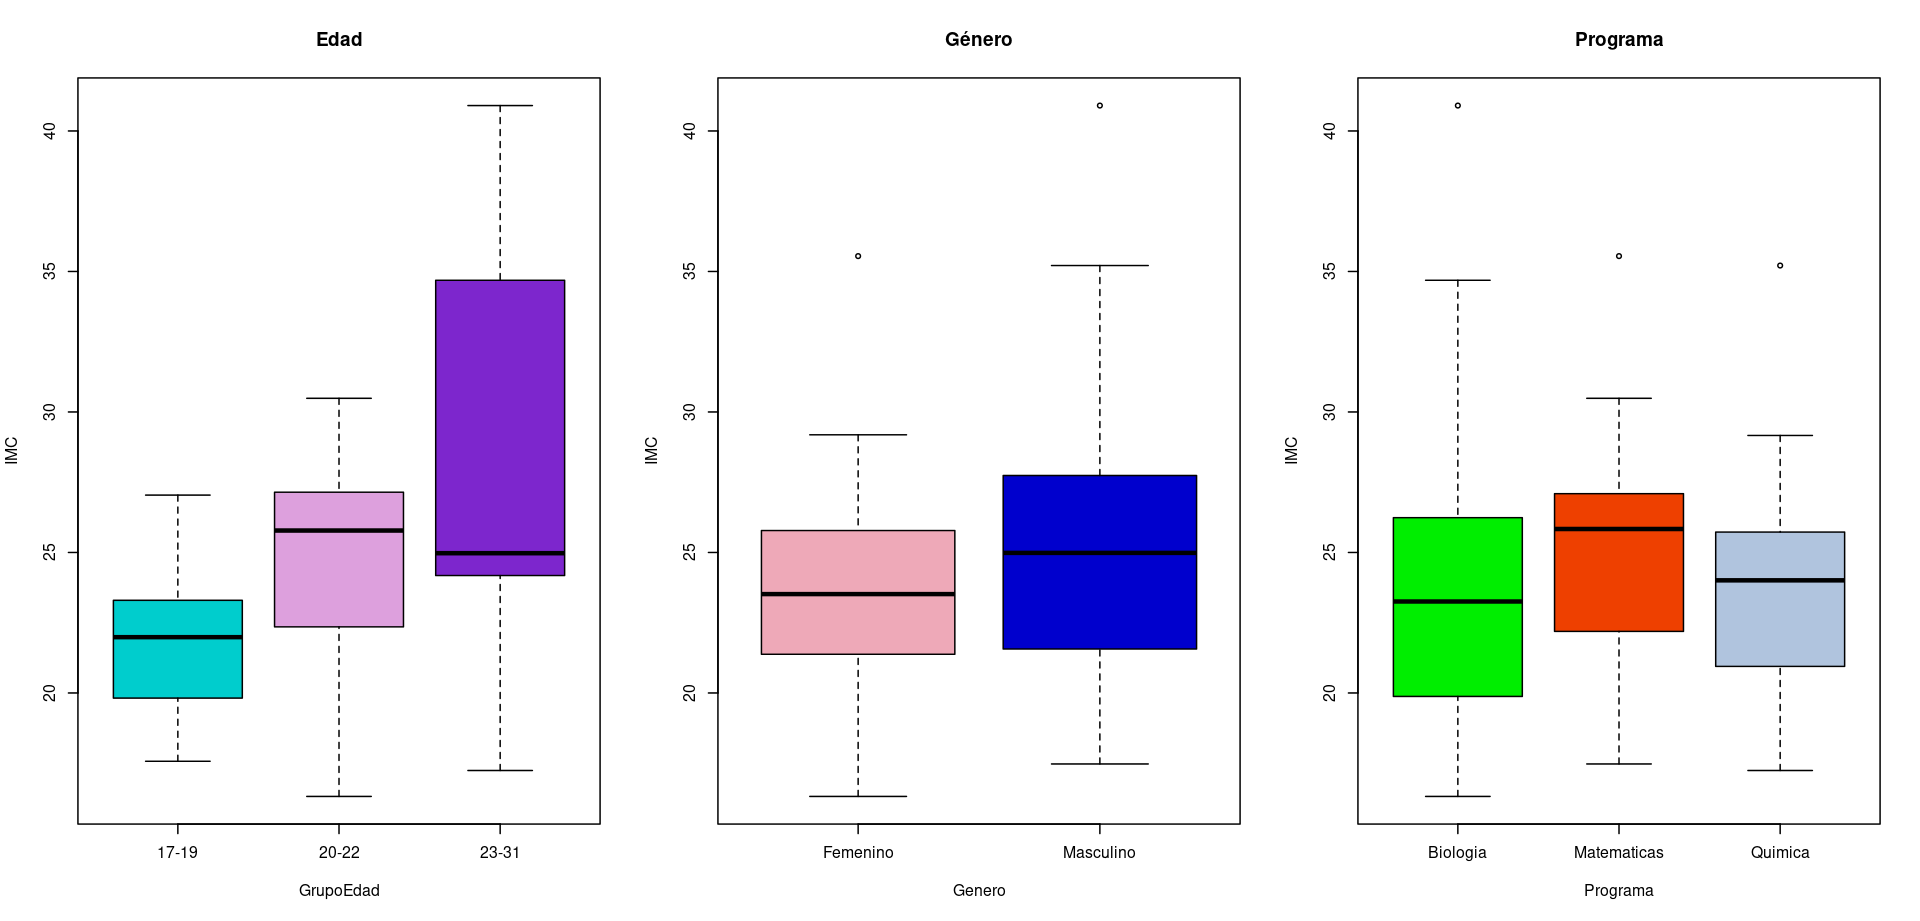
\includegraphics[width=1\textwidth]{Boxplot-IMC.png}
    \caption{Boxplots del IMC según grupo de edad, género y programa académico. Este gráfico permite comparar visualmente la distribución y variabilidad del índice de masa corporal entre los distintos niveles de cada factor.}
    \label{fig:boxplots_imc}
\end{figure}

En la figura se presentan diagramas de caja (boxplots) que muestran la distribución del IMC según los factores \texttt{GrupoEdad}, \texttt{Género} y \texttt{Programa}. Estos gráficos permiten observar visualmente las diferencias en las medianas, la dispersión y la presencia de valores atípicos.

\begin{itemize}
    \item \textbf{GrupoEdad:} Se aprecia un aumento del IMC con la edad. El grupo de 23--31 años muestra mayor variabilidad y una mediana más alta. Los grupos de menor edad presentan distribuciones más compactas.
    
    \item \textbf{Género:} La mediana del IMC es ligeramente mayor en el grupo masculino. También se observa una mayor dispersión en este grupo y la presencia de valores atípicos altos.

    \item \textbf{Programa:} Las medianas son similares entre los programas de Biología, Matemáticas y Química. No se evidencian diferencias marcadas en las distribuciones, aunque Biología presenta una mayor variabilidad.
\end{itemize}
\subsubsection{Análisis de varianza}
Dado que se cumplen todos los supuestos podemos realizar el ANOVA. Con lo cual, empleamos el siguiente comando: 

\begin{lstlisting}[style=rstyle]
    summary(Modelo)
\end{lstlisting}

Obteniendo los siguientes resultados :

\begin{verbatim}
                           Df Sum Sq Mean Sq F value  Pr(>F)    
Programa                   2   20.2   10.12   0.730 0.487649    
Genero                     1   48.3   48.32   3.488 0.068629 .  
GrupoEdad                  2  310.3  155.16  11.202 0.000121 ***
Programa:Genero            2    6.2    3.12   0.225 0.799521    
Programa:GrupoEdad         4  212.1   53.03   3.829 0.009504 ** 
Genero:GrupoEdad           2    4.2    2.08   0.150 0.860838    
Programa:Genero:GrupoEdad  3  140.4   46.81   3.380 0.026665 *  
Residuals                 43  595.6   13.85                     
---
Signif. codes:  0 ‘***’ 0.001 ‘**’ 0.01 ‘*’ 0.05 ‘.’ 0.1 ‘ ’ 1
\end{verbatim}

El Análisis de Varianza (ANOVA) es una técnica estadística utilizada para determinar si existen diferencias significativas entre las medias de varios grupos. Se aplica cuando la variable dependiente es cuantitativa (por ejemplo, IMC), y se desea estudiar su comportamiento según uno o varios factores categóricos (como Programa, Género y GrupoEdad).\\

El ANOVA evalúa las siguientes hipótesis:

\begin{itemize}
    \item \( H_0 \): Las medias de todos los grupos son iguales.
    \item \( H_1 \): Al menos una media de grupo difiere de las demás.
\end{itemize}

Para ello, el ANOVA compara la variabilidad explicada por los factores del modelo con la variabilidad residual (error) mediante el estadístico F. Un valor-p pequeño (menor a 0.05) indica evidencia significativa para rechazar la hipótesis nula, lo que implica que el factor tiene un efecto sobre la variable de interés.\\

En este caso, el ANOVA permite determinar si el IMC varía de manera significativa según el Programa, el Género, el Grupo de Edad y sus posibles interacciones.

\begin{itemize}
    \item \textbf{Programa : }valor-p = 0.4876 es mayor que 0.05. Luego, el IMC no varía significativamente entre programas.
    
    \item \textbf{Género : }valor-p = 0.068629, esta cerca de 0.05. Luego, el género podría influir levemente en el IMC.
    
    \item \textbf{GrupoEdad :} valor-p = 0.000121 es menor que 0.05. Luego, el IMC varía significativamente entre grupos de edad.
    
    \item \textbf{Programa × Género :} valor-p = 0.799521 es mayor que 0.05. Luego, no hay interacción entre programa y género.
    
    \item \textbf{Programa × GrupoEdad :} valor-p = 0.009504 es menor que 0.05. Luego, el efecto del programa sobre el IMC depende del grupo de edad.
    
    \item \textbf{Género × GrupoEdad :} valor-p = 0.860838 es mayor que 0.05. Luego, no hay interacción entre género y grupo de edad.
    
    \item \textbf{Programa × Género × GrupoEdad:} valor-p = 0.026665 es menor que 0.05. Luego, hay una interacción significativa entre los tres factores.
\end{itemize}

\subsubsection{Prueba de medias}
Para los casos donde se evidencia una diferencia significativa realizaremos la prueba de medias, es decir, para GrupoEdad, Programa × GrupoEdad y Programa × Género × GrupoEdad. Para esto, realizaremos la prueba de Turkey en cada una de ellas. \\

La prueba de Tukey, también conocida como la prueba de comparaciones múltiples de Tukey o HSD (Honestly Significant Difference), es un método estadístico utilizado para realizar comparaciones por pares entre medias cuando se ha detectado una diferencia significativa en un análisis de varianza (ANOVA). Su objetivo principal es identificar exactamente cuáles grupos difieren entre sí, controlando el error tipo I (falso positivo) en múltiples comparaciones.

\begin{itemize}
    \item[$\diamond$] Se basa en la diferencia entre todas las pares de medias de los grupos comparados.
    \item[$\diamond$] Calcula un umbral (valor crítico) que determina si la diferencia entre dos medias es estadísticamente significativa.
    \item[$\diamond$] Si la diferencia entre las medias de dos grupos excede este valor crítico, se concluye que esas medias difieren de manera significativa.
\end{itemize}

\textbf{Ventajas:}

\begin{itemize}
    \item[$\diamond$] Controla la tasa de error tipo I en comparaciones múltiples.
    \item[$\diamond$] Es apropiada cuando se comparan todos los pares posibles de grupos.
\end{itemize}

\begin{itemize}
    \item \textbf{Prueba de Turkey en GrupoEdad :} Para realizar dicha prueba, empleamos el siguiente código

\begin{lstlisting}[style=rstyle]
TukeyHSD(Modelo, "GrupoEdad")
\end{lstlisting}

    Obteniendo los siguientes resultados:

    \begin{verbatim}
        Tukey multiple comparisons of means
    95% family-wise confidence level

Fit: aov(formula = IMC ~ Programa * Genero * GrupoEdad,
data = CienciasExactasIMC)

$GrupoEdad
                diff        lwr      upr     p adj
20-22-17-19 2.459628 -0.2511832 5.170440 0.0821312
23-31-17-19 5.872434  2.5842320 9.160637 0.0002501
23-31-20-22 3.412806  0.3974432 6.428169 0.0232930
    \end{verbatim}
El grupo 23–31 años tiene un IMC significativamente mayor que el grupo 17–19 años (p = 0.00025) y el grupo 20–22 años (p = 0.0233). Mientras que, la diferencia entre 20–22 y 17–19 años no es significativa (p = 0.0821).

\begin{figure}[H]
    \centering
    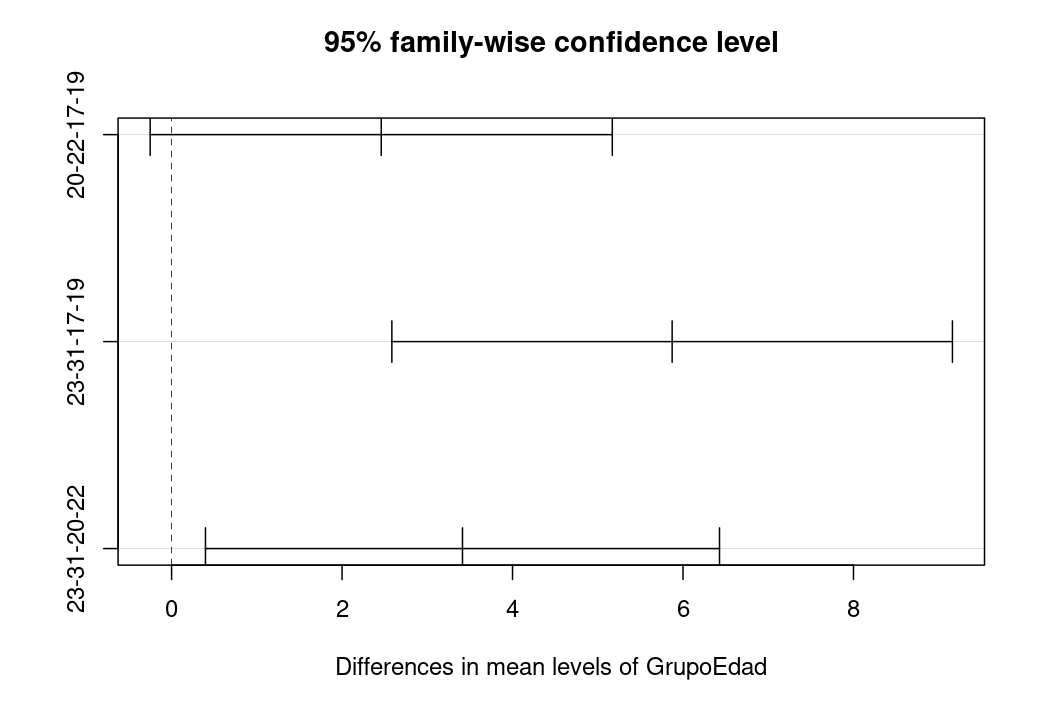
\includegraphics[width=0.8\textwidth]{turkey_GrupoEdad.png}
    \caption{Intervalos de confianza del 95\% para las diferencias en los niveles medios de IMC entre grupos de edad. Solo la comparación entre los grupos 23-31 y 17-19 muestra una diferencia significativa.}
\end{figure}

\item \textbf{Prueba de Turkey en Programa × GrupoEdad :} Para realizar dicha prueba, empleamos el siguiente código
\begin{verbatim}
    TukeyHSD(Modelo, "Programa:GrupoEdad")
\end{verbatim}

Obteniendo los siguientes resultados:

\begin{verbatim}
    Tukey multiple comparisons of means
    95% family-wise confidence level

Fit: aov(formula = IMC ~ Programa * Genero * GrupoEdad, 
data = CienciasExactasIMC)

$`Programa:GrupoEdad`
                                            diff         lwr
Matematicas:17-19-Biologia:17-19      1.99176343  -7.2875711
Quimica:17-19-Biologia:17-19          0.58226648  -6.4322511
Biologia:20-22-Biologia:17-19         3.97379401  -2.1009564
Matematicas:20-22-Biologia:17-19      3.05843042  -1.7211576
Quimica:20-22-Biologia:17-19          2.96038935  -2.3970369
Biologia:23-31-Biologia:17-19        15.31887201   6.0395375
Matematicas:23-31-Biologia:17-19      7.60102888   0.5865113
Quimica:23-31-Biologia:17-19          3.15033360  -2.6279066
Quimica:17-19-Matematicas:17-19      -1.40949695 -11.9312733
Biologia:20-22-Matematicas:17-19      1.98203057  -7.9379953
Matematicas:20-22-Matematicas:17-19   1.06666698  -8.1174923
Quimica:20-22-Matematicas:17-19       0.96862592  -8.5290757
Biologia:23-31-Matematicas:17-19     13.32710857   1.1776078
Matematicas:23-31-Matematicas:17-19   5.60926545  -4.9125109
Quimica:23-31-Matematicas:17-19       1.15857017  -8.5827018
Biologia:20-22-Quimica:17-19          3.39152752  -4.4509415
Matematicas:20-22-Quimica:17-19       2.47616393  -4.4119556
Quimica:20-22-Quimica:17-19           2.37812287  -4.9228185
Biologia:23-31-Quimica:17-19         14.73660552   4.2148292
Matematicas:23-31-Quimica:17-19       7.01876240  -1.5722320
Quimica:23-31-Quimica:17-19           2.56806711  -5.0470355
Matematicas:20-22-Biologia:20-22     -0.91536359  -6.8437129
Quimica:20-22-Biologia:20-22         -1.01340466  -7.4167538
Biologia:23-31-Biologia:20-22        11.34507800   1.4250521
Matematicas:23-31-Biologia:20-22      3.62723488  -4.2152342
Quimica:23-31-Biologia:20-22         -0.82346041  -7.5828187
Quimica:20-22-Matematicas:20-22      -0.09804107  -5.2888743
Biologia:23-31-Matematicas:20-22     12.26044159   3.0762823
Matematicas:23-31-Matematicas:20-22   4.54259847  -2.3455210
Quimica:23-31-Matematicas:20-22       0.09190318  -5.5322228
Biologia:23-31-Quimica:20-22         12.35848266   2.8607810
Matematicas:23-31-Quimica:20-22       4.64063953  -2.6603018
Quimica:23-31-Quimica:20-22           0.18994425  -5.9328286
Matematicas:23-31-Biologia:23-31     -7.71784312 -18.2396195
Quimica:23-31-Biologia:23-31        -12.16853841 -21.9098104
Quimica:23-31-Matematicas:23-31      -4.45069528 -12.0657979

                                          
                                          upr     p adj
Matematicas:17-19-Biologia:17-19    11.271098 0.9985288
Quimica:17-19-Biologia:17-19         7.596784 0.9999989
Biologia:20-22-Biologia:17-19       10.048544 0.4640342
Matematicas:20-22-Biologia:17-19     7.838018 0.4937627
Quimica:20-22-Biologia:17-19         8.317816 0.6793669
Biologia:23-31-Biologia:17-19       24.598207 0.0000915
Matematicas:23-31-Biologia:17-19    14.615546 0.0248126
Quimica:23-31-Biologia:17-19         8.928574 0.6945074
Quimica:17-19-Matematicas:17-19      9.112279 0.9999553
Biologia:20-22-Matematicas:17-19    11.902056 0.9991194
Matematicas:20-22-Matematicas:17-19 10.250826 0.9999851
Quimica:20-22-Matematicas:17-19     10.466328 0.9999946
Biologia:23-31-Matematicas:17-19    25.476609 0.0220982
Matematicas:23-31-Matematicas:17-19 16.131042 0.7189014
Quimica:23-31-Matematicas:17-19     10.899842 0.9999821
Biologia:20-22-Quimica:17-19        11.233997 0.8871134
Matematicas:20-22-Quimica:17-19      9.364283 0.9578507
Quimica:20-22-Quimica:17-19          9.679064 0.9764496
Biologia:23-31-Quimica:17-19        25.258382 0.0012346
Matematicas:23-31-Quimica:17-19     15.609757 0.1902195
Quimica:23-31-Quimica:17-19         10.183170 0.9709784
Matematicas:20-22-Biologia:20-22     5.012986 0.9998687
Quimica:20-22-Biologia:20-22         5.389945 0.9998419
Biologia:23-31-Biologia:20-22       21.265104 0.0145907
Matematicas:23-31-Biologia:20-22    11.469704 0.8447640
Quimica:23-31-Biologia:20-22         5.935898 0.9999784
Quimica:20-22-Matematicas:20-22      5.092792 1.0000000
Biologia:23-31-Matematicas:20-22    21.444601 0.0023786
Matematicas:23-31-Matematicas:20-22 11.430718 0.4530583
Quimica:23-31-Matematicas:20-22      5.716029 1.0000000
Biologia:23-31-Quimica:20-22        21.856184 0.0033131
Matematicas:23-31-Quimica:20-22     11.941581 0.5027675
Quimica:23-31-Quimica:20-22          6.312717 1.0000000
Matematicas:23-31-Biologia:23-31     2.803933 0.3127987
Quimica:23-31-Biologia:23-31        -2.427266 0.0054744
Quimica:23-31-Matematicas:23-31      3.164407 0.6121724
   
    \end{verbatim}

Las comparaciones con diferencias estadísticamente significativas (\(p\text{-valor} < 0.05\)) son las siguientes:

\begin{itemize}
    \item Biología:23--31 vs Biología:17--19 (\(p = 0.00009\))
    \item Matemáticas:23--31 vs Biología:17--19 (\(p = 0.02481\))
    \item Biología:23--31 vs Matemáticas:17--19 (\(p = 0.02210\))
    \item Biología:23--31 vs Química:17--19 (\(p = 0.00123\))
    \item Biología:23--31 vs Biología:20--22 (\(p = 0.01459\))
    \item Biología:23--31 vs Matemáticas:20--22 (\(p = 0.00237\))
    \item Biología:23--31 vs Química:20--22 (\(p = 0.00331\))
    \item Química:23--31 vs Biología:23--31 (\(p = 0.00547\))
\end{itemize}

En general, se observa que el grupo \texttt{Biología:23--31} presenta un IMC significativamente más alto en comparación con múltiples combinaciones de niveles más jóvenes, lo cual coincide con lo observado en los diagramas de caja. 

\begin{figure}[H]
    \centering
    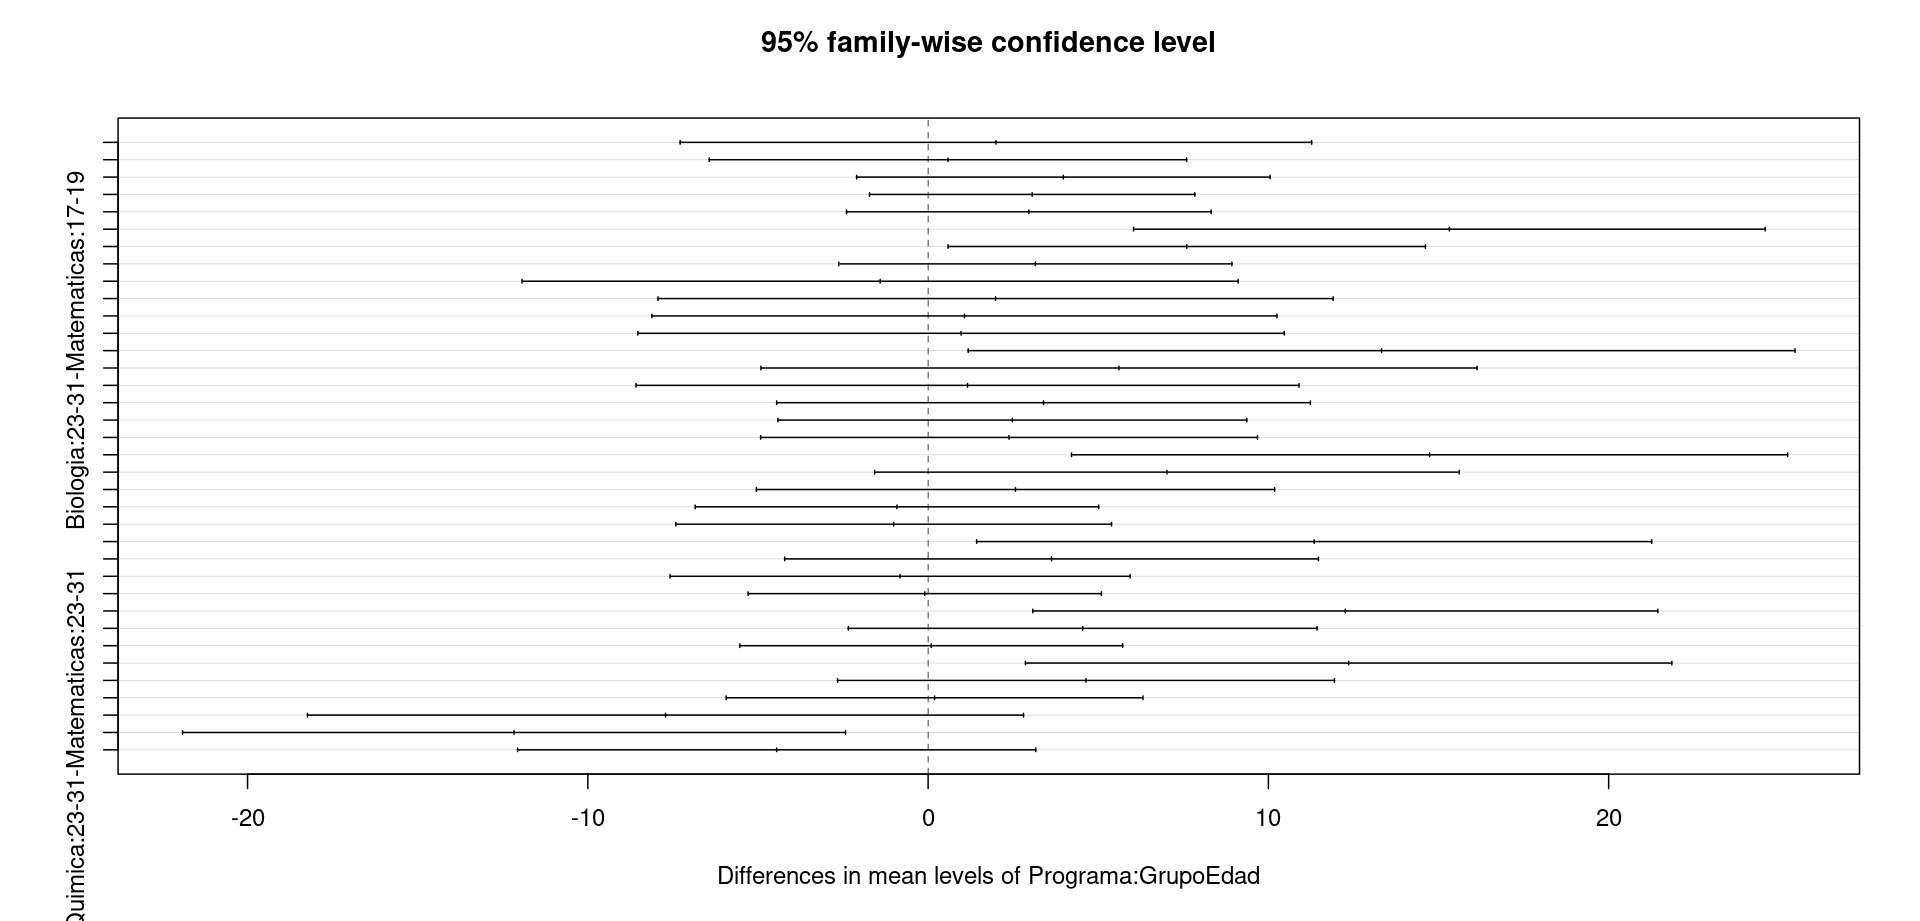
\includegraphics[width=1.0\textwidth]{turkey_Programa-GrupoEdad.png}
    \caption{Intervalos de confianza del 95\% para las diferencias en los niveles medios de IMC según la interacción Programa × GrupoEdad. .}
\end{figure}

\item \textbf{Prueba de Turkey en Programa × Género × GrupoEdad: }Para realizar dicha prueba, empleamos el siguiente código

\begin{verbatim}
    TukeyHSD(Modelo, "Programa:Genero:GrupoEdad")
\end{verbatim}

Obteniendo los siguientes resultados:

\begin{verbatim}
 Tukey multiple comparisons of means
    95% family-wise confidence level

Fit: aov(formula = IMC ~ Programa * Genero * GrupoEdad, data = CienciasExactasIMC)

$`Programa:Genero:GrupoEdad`
                                                                diff
Matematicas:Femenino:17-19-Biologia:Femenino:17-19       -2.36496183
Quimica:Femenino:17-19-Biologia:Femenino:17-19           -1.45944559
Biologia:Masculino:17-19-Biologia:Femenino:17-19         -1.52047528
Matematicas:Masculino:17-19-Biologia:Femenino:17-19       4.85883781
Quimica:Masculino:17-19-Biologia:Femenino:17-19           1.58862225
Biologia:Femenino:20-22-Biologia:Femenino:17-19           0.95114707
Matematicas:Femenino:20-22-Biologia:Femenino:17-19        1.51864778
Quimica:Femenino:20-22-Biologia:Femenino:17-19            5.42207480
Biologia:Masculino:20-22-Biologia:Femenino:17-19          6.54430116
Matematicas:Masculino:20-22-Biologia:Femenino:17-19       2.99449006
Quimica:Masculino:20-22-Biologia:Femenino:17-19           2.07608814
Biologia:Femenino:23-31-Biologia:Femenino:17-19                   NA
Matematicas:Femenino:23-31-Biologia:Femenino:17-19        7.53247961
Quimica:Femenino:23-31-Biologia:Femenino:17-19            0.31846003
Biologia:Masculino:23-31-Biologia:Femenino:17-19         15.61255251
Matematicas:Masculino:23-31-Biologia:Femenino:17-19       3.56148214
Quimica:Masculino:23-31-Biologia:Femenino:17-19           5.68024447
Quimica:Femenino:17-19-Matematicas:Femenino:17-19         0.90551623
Biologia:Masculino:17-19-Matematicas:Femenino:17-19       0.84448655
Matematicas:Masculino:17-19-Matematicas:Femenino:17-19    7.22379964
Quimica:Masculino:17-19-Matematicas:Femenino:17-19        3.95358408
Biologia:Femenino:20-22-Matematicas:Femenino:17-19        3.31610889
Matematicas:Femenino:20-22-Matematicas:Femenino:17-19     3.88360961
Quimica:Femenino:20-22-Matematicas:Femenino:17-19         7.78703662
Biologia:Masculino:20-22-Matematicas:Femenino:17-19       8.90926299
Matematicas:Masculino:20-22-Matematicas:Femenino:17-19    5.35945189
Quimica:Masculino:20-22-Matematicas:Femenino:17-19        4.44104997
Biologia:Femenino:23-31-Matematicas:Femenino:17-19                NA
Matematicas:Femenino:23-31-Matematicas:Femenino:17-19     9.89744144
Quimica:Femenino:23-31-Matematicas:Femenino:17-19         2.68342186
Biologia:Masculino:23-31-Matematicas:Femenino:17-19      17.97751433
Matematicas:Masculino:23-31-Matematicas:Femenino:17-19    5.92644397
Quimica:Masculino:23-31-Matematicas:Femenino:17-19        8.04520630
Biologia:Masculino:17-19-Quimica:Femenino:17-19          -0.06102968
Matematicas:Masculino:17-19-Quimica:Femenino:17-19        6.31828341
Quimica:Masculino:17-19-Quimica:Femenino:17-19            3.04806785
Biologia:Femenino:20-22-Quimica:Femenino:17-19            2.41059266
Matematicas:Femenino:20-22-Quimica:Femenino:17-19         2.97809337
Quimica:Femenino:20-22-Quimica:Femenino:17-19             6.88152039
Biologia:Masculino:20-22-Quimica:Femenino:17-19           8.00374676
Matematicas:Masculino:20-22-Quimica:Femenino:17-19        4.45393566
Quimica:Masculino:20-22-Quimica:Femenino:17-19            3.53553374
Biologia:Femenino:23-31-Quimica:Femenino:17-19                    NA
Matematicas:Femenino:23-31-Quimica:Femenino:17-19         8.99192520
Quimica:Femenino:23-31-Quimica:Femenino:17-19             1.77790563
Biologia:Masculino:23-31-Quimica:Femenino:17-19          17.07199810
Matematicas:Masculino:23-31-Quimica:Femenino:17-19        5.02092774
Quimica:Masculino:23-31-Quimica:Femenino:17-19            7.13969007
Matematicas:Masculino:17-19-Biologia:Masculino:17-19      6.37931309
Quimica:Masculino:17-19-Biologia:Masculino:17-19          3.10909753
Biologia:Femenino:20-22-Biologia:Masculino:17-19          2.47162234
Matematicas:Femenino:20-22-Biologia:Masculino:17-19       3.03912306
Quimica:Femenino:20-22-Biologia:Masculino:17-19           6.94255007
Biologia:Masculino:20-22-Biologia:Masculino:17-19         8.06477644
Matematicas:Masculino:20-22-Biologia:Masculino:17-19      4.51496534
Quimica:Masculino:20-22-Biologia:Masculino:17-19          3.59656342
Biologia:Femenino:23-31-Biologia:Masculino:17-19                  NA
Matematicas:Femenino:23-31-Biologia:Masculino:17-19       9.05295488
Quimica:Femenino:23-31-Biologia:Masculino:17-19           1.83893531
Biologia:Masculino:23-31-Biologia:Masculino:17-19        17.13302778
Matematicas:Masculino:23-31-Biologia:Masculino:17-19      5.08195742
Quimica:Masculino:23-31-Biologia:Masculino:17-19          7.20071975
Quimica:Masculino:17-19-Matematicas:Masculino:17-19      -3.27021556
Biologia:Femenino:20-22-Matematicas:Masculino:17-19      -3.90769075
Matematicas:Femenino:20-22-Matematicas:Masculino:17-19   -3.34019003
Quimica:Femenino:20-22-Matematicas:Masculino:17-19        0.56323699
Biologia:Masculino:20-22-Matematicas:Masculino:17-19      1.68546335
Matematicas:Masculino:20-22-Matematicas:Masculino:17-19  -1.86434775
Quimica:Masculino:20-22-Matematicas:Masculino:17-19      -2.78274967
Biologia:Femenino:23-31-Matematicas:Masculino:17-19               NA
Matematicas:Femenino:23-31-Matematicas:Masculino:17-19    2.67364180
Quimica:Femenino:23-31-Matematicas:Masculino:17-19       -4.54037778
Biologia:Masculino:23-31-Matematicas:Masculino:17-19     10.75371470
Matematicas:Masculino:23-31-Matematicas:Masculino:17-19  -1.29735567
Quimica:Masculino:23-31-Matematicas:Masculino:17-19       0.82140666
Biologia:Femenino:20-22-Quimica:Masculino:17-19          -0.63747518
Matematicas:Femenino:20-22-Quimica:Masculino:17-19       -0.06997447
Quimica:Femenino:20-22-Quimica:Masculino:17-19            3.83345255
Biologia:Masculino:20-22-Quimica:Masculino:17-19          4.95567891
Matematicas:Masculino:20-22-Quimica:Masculino:17-19       1.40586781
Quimica:Masculino:20-22-Quimica:Masculino:17-19           0.48746589
Biologia:Femenino:23-31-Quimica:Masculino:17-19                   NA
Matematicas:Femenino:23-31-Quimica:Masculino:17-19        5.94385736
Quimica:Femenino:23-31-Quimica:Masculino:17-19           -1.27016222
Biologia:Masculino:23-31-Quimica:Masculino:17-19         14.02393026
Matematicas:Masculino:23-31-Quimica:Masculino:17-19       1.97285989
Quimica:Masculino:23-31-Quimica:Masculino:17-19           4.09162222
Matematicas:Femenino:20-22-Biologia:Femenino:20-22        0.56750071
Quimica:Femenino:20-22-Biologia:Femenino:20-22            4.47092773
Biologia:Masculino:20-22-Biologia:Femenino:20-22          5.59315409
Matematicas:Masculino:20-22-Biologia:Femenino:20-22       2.04334299
Quimica:Masculino:20-22-Biologia:Femenino:20-22           1.12494108
Biologia:Femenino:23-31-Biologia:Femenino:20-22                   NA
Matematicas:Femenino:23-31-Biologia:Femenino:20-22        6.58133254
Quimica:Femenino:23-31-Biologia:Femenino:20-22           -0.63268703
Biologia:Masculino:23-31-Biologia:Femenino:20-22         14.66140544
Matematicas:Masculino:23-31-Biologia:Femenino:20-22       2.61033508
Quimica:Masculino:23-31-Biologia:Femenino:20-22           4.72909741
Quimica:Femenino:20-22-Matematicas:Femenino:20-22         3.90342702
Biologia:Masculino:20-22-Matematicas:Femenino:20-22       5.02565338
Matematicas:Masculino:20-22-Matematicas:Femenino:20-22    1.47584228
Quimica:Masculino:20-22-Matematicas:Femenino:20-22        0.55744036
Biologia:Femenino:23-31-Matematicas:Femenino:20-22                NA
Matematicas:Femenino:23-31-Matematicas:Femenino:20-22     6.01383183
Quimica:Femenino:23-31-Matematicas:Femenino:20-22        -1.20018775
Biologia:Masculino:23-31-Matematicas:Femenino:20-22      14.09390473
Matematicas:Masculino:23-31-Matematicas:Femenino:20-22    2.04283436
Quimica:Masculino:23-31-Matematicas:Femenino:20-22        4.16159669
Biologia:Masculino:20-22-Quimica:Femenino:20-22           1.12222636
Matematicas:Masculino:20-22-Quimica:Femenino:20-22       -2.42758474
Quimica:Masculino:20-22-Quimica:Femenino:20-22           -3.34598665
Biologia:Femenino:23-31-Quimica:Femenino:20-22                    NA
Matematicas:Femenino:23-31-Quimica:Femenino:20-22         2.11040481
Quimica:Femenino:23-31-Quimica:Femenino:20-22            -5.10361476
Biologia:Masculino:23-31-Quimica:Femenino:20-22          10.19047771
Matematicas:Masculino:23-31-Quimica:Femenino:20-22       -1.86059266
Quimica:Masculino:23-31-Quimica:Femenino:20-22            0.25816967
Matematicas:Masculino:20-22-Biologia:Masculino:20-22     -3.54981110
Quimica:Masculino:20-22-Biologia:Masculino:20-22         -4.46821302
Biologia:Femenino:23-31-Biologia:Masculino:20-22                  NA
Matematicas:Femenino:23-31-Biologia:Masculino:20-22       0.98817845
Quimica:Femenino:23-31-Biologia:Masculino:20-22          -6.22584113
Biologia:Masculino:23-31-Biologia:Masculino:20-22         9.06825135
Matematicas:Masculino:23-31-Biologia:Masculino:20-22     -2.98281902
Quimica:Masculino:23-31-Biologia:Masculino:20-22         -0.86405669
Quimica:Masculino:20-22-Matematicas:Masculino:20-22      -0.91840192
Biologia:Femenino:23-31-Matematicas:Masculino:20-22               NA
Matematicas:Femenino:23-31-Matematicas:Masculino:20-22    4.53798955
Quimica:Femenino:23-31-Matematicas:Masculino:20-22       -2.67603003
Biologia:Masculino:23-31-Matematicas:Masculino:20-22     12.61806245
Matematicas:Masculino:23-31-Matematicas:Masculino:20-22   0.56699208
Quimica:Masculino:23-31-Matematicas:Masculino:20-22       2.68575441
Biologia:Femenino:23-31-Quimica:Masculino:20-22                   NA
Matematicas:Femenino:23-31-Quimica:Masculino:20-22        5.45639147
Quimica:Femenino:23-31-Quimica:Masculino:20-22           -1.75762811
Biologia:Masculino:23-31-Quimica:Masculino:20-22         13.53646436
Matematicas:Masculino:23-31-Quimica:Masculino:20-22       1.48539400
Quimica:Masculino:23-31-Quimica:Masculino:20-22           3.60415633
Matematicas:Femenino:23-31-Biologia:Femenino:23-31                NA
Quimica:Femenino:23-31-Biologia:Femenino:23-31                    NA
Biologia:Masculino:23-31-Biologia:Femenino:23-31                  NA
Matematicas:Masculino:23-31-Biologia:Femenino:23-31               NA
Quimica:Masculino:23-31-Biologia:Femenino:23-31                   NA
Quimica:Femenino:23-31-Matematicas:Femenino:23-31        -7.21401958
Biologia:Masculino:23-31-Matematicas:Femenino:23-31       8.08007290
Matematicas:Masculino:23-31-Matematicas:Femenino:23-31   -3.97099747
Quimica:Masculino:23-31-Matematicas:Femenino:23-31       -1.85223514
Biologia:Masculino:23-31-Quimica:Femenino:23-31          15.29409247
Matematicas:Masculino:23-31-Quimica:Femenino:23-31        3.24302211
Quimica:Masculino:23-31-Quimica:Femenino:23-31            5.36178444
Matematicas:Masculino:23-31-Biologia:Masculino:23-31    -12.05107037
Quimica:Masculino:23-31-Biologia:Masculino:23-31         -9.93230804
Quimica:Masculino:23-31-Matematicas:Masculino:23-31       2.11876233
                                                                lwr
Matematicas:Femenino:17-19-Biologia:Femenino:17-19      -17.2671101
Quimica:Femenino:17-19-Biologia:Femenino:17-19          -11.2151917
Biologia:Masculino:17-19-Biologia:Femenino:17-19         -9.4860086
Matematicas:Masculino:17-19-Biologia:Femenino:17-19     -10.0433105
Quimica:Masculino:17-19-Biologia:Femenino:17-19         -13.3135260
Biologia:Femenino:20-22-Biologia:Femenino:17-19          -7.9545899
Matematicas:Femenino:20-22-Biologia:Femenino:17-19       -6.4468855
Quimica:Femenino:20-22-Biologia:Femenino:17-19           -5.8428905
Biologia:Masculino:20-22-Biologia:Femenino:17-19         -4.7206641
Matematicas:Masculino:20-22-Biologia:Femenino:17-19      -4.4565841
Quimica:Masculino:20-22-Biologia:Femenino:17-19          -5.5996918
Biologia:Femenino:23-31-Biologia:Femenino:17-19                  NA
Matematicas:Femenino:23-31-Biologia:Femenino:17-19       -2.2232665
Quimica:Femenino:23-31-Biologia:Femenino:17-19           -8.0358618
Biologia:Masculino:23-31-Biologia:Femenino:17-19          4.3475872
Matematicas:Masculino:23-31-Biologia:Femenino:17-19     -11.3406662
Quimica:Masculino:23-31-Biologia:Femenino:17-19          -5.5847208
Quimica:Femenino:17-19-Matematicas:Femenino:17-19       -15.0255504
Biologia:Masculino:17-19-Matematicas:Femenino:17-19     -14.0576617
Matematicas:Masculino:17-19-Matematicas:Femenino:17-19  -12.2876925
Quimica:Masculino:17-19-Matematicas:Femenino:17-19      -15.5579081
Biologia:Femenino:20-22-Matematicas:Femenino:17-19      -12.1090801
Matematicas:Femenino:20-22-Matematicas:Femenino:17-19   -11.0185387
Quimica:Femenino:20-22-Matematicas:Femenino:17-19        -9.1104113
Biologia:Masculino:20-22-Matematicas:Femenino:17-19      -7.9881849
Matematicas:Masculino:20-22-Matematicas:Femenino:17-19   -9.2741672
Quimica:Masculino:20-22-Matematicas:Femenino:17-19      -10.3082517
Biologia:Femenino:23-31-Matematicas:Femenino:17-19               NA
Matematicas:Femenino:23-31-Matematicas:Femenino:17-19    -6.0336252
Quimica:Femenino:23-31-Matematicas:Femenino:17-19       -12.4301150
Biologia:Masculino:23-31-Matematicas:Femenino:17-19       1.0800664
Matematicas:Masculino:23-31-Matematicas:Femenino:17-19  -13.5850482
Quimica:Masculino:23-31-Matematicas:Femenino:17-19       -8.8522416
Biologia:Masculino:17-19-Quimica:Femenino:17-19          -9.8167758
Matematicas:Masculino:17-19-Quimica:Femenino:17-19       -9.6127832
Quimica:Masculino:17-19-Quimica:Femenino:17-19          -12.8829988
Biologia:Femenino:20-22-Quimica:Femenino:17-19           -8.1268175
Matematicas:Femenino:20-22-Quimica:Femenino:17-19        -6.7776527
Quimica:Femenino:20-22-Quimica:Femenino:17-19            -5.7130936
Biologia:Masculino:20-22-Quimica:Femenino:17-19          -4.5908673
Matematicas:Masculino:20-22-Quimica:Femenino:17-19       -4.8864801
Quimica:Masculino:20-22-Quimica:Femenino:17-19           -5.9850996
Biologia:Femenino:23-31-Quimica:Femenino:17-19                   NA
Matematicas:Femenino:23-31-Quimica:Femenino:17-19        -2.2730401
Quimica:Femenino:23-31-Quimica:Femenino:17-19            -8.2977856
Biologia:Masculino:23-31-Quimica:Femenino:17-19           4.4773841
Matematicas:Masculino:23-31-Quimica:Femenino:17-19      -10.9101389
Quimica:Masculino:23-31-Quimica:Femenino:17-19           -5.4549240
Matematicas:Masculino:17-19-Biologia:Masculino:17-19     -8.5228352
Quimica:Masculino:17-19-Biologia:Masculino:17-19        -11.7930508
Biologia:Femenino:20-22-Biologia:Masculino:17-19         -6.4341147
Matematicas:Femenino:20-22-Biologia:Masculino:17-19      -4.9264103
Quimica:Femenino:20-22-Biologia:Masculino:17-19          -4.3224152
Biologia:Masculino:20-22-Biologia:Masculino:17-19        -3.2001888
Matematicas:Masculino:20-22-Biologia:Masculino:17-19     -2.9361088
Quimica:Masculino:20-22-Biologia:Masculino:17-19         -4.0792166
Biologia:Femenino:23-31-Biologia:Masculino:17-19                 NA
Matematicas:Femenino:23-31-Biologia:Masculino:17-19      -0.7027912
Quimica:Femenino:23-31-Biologia:Masculino:17-19          -6.5153865
Biologia:Masculino:23-31-Biologia:Masculino:17-19         5.8680625
Matematicas:Masculino:23-31-Biologia:Masculino:17-19     -9.8201909
Quimica:Masculino:23-31-Biologia:Masculino:17-19         -4.0642455
Quimica:Masculino:17-19-Matematicas:Masculino:17-19     -22.7817077
Biologia:Femenino:20-22-Matematicas:Masculino:17-19     -19.3328797
Matematicas:Femenino:20-22-Matematicas:Masculino:17-19  -18.2423383
Quimica:Femenino:20-22-Matematicas:Masculino:17-19      -16.3342109
Biologia:Masculino:20-22-Matematicas:Masculino:17-19    -15.2119845
Matematicas:Masculino:20-22-Matematicas:Masculino:17-19 -16.4979669
Quimica:Masculino:20-22-Matematicas:Masculino:17-19     -17.5320514
Biologia:Femenino:23-31-Matematicas:Masculino:17-19              NA
Matematicas:Femenino:23-31-Matematicas:Masculino:17-19  -13.2574249
Quimica:Femenino:23-31-Matematicas:Masculino:17-19      -19.6539146
Biologia:Masculino:23-31-Matematicas:Masculino:17-19     -6.1437332
Matematicas:Masculino:23-31-Matematicas:Masculino:17-19 -20.8088478
Quimica:Masculino:23-31-Matematicas:Masculino:17-19     -16.0760412
Biologia:Femenino:20-22-Quimica:Masculino:17-19         -16.0626641
Matematicas:Femenino:20-22-Quimica:Masculino:17-19      -14.9721228
Quimica:Femenino:20-22-Quimica:Masculino:17-19          -13.0639953
Biologia:Masculino:20-22-Quimica:Masculino:17-19        -11.9417690
Matematicas:Masculino:20-22-Quimica:Masculino:17-19     -13.2277513
Quimica:Masculino:20-22-Quimica:Masculino:17-19         -14.2618358
Biologia:Femenino:23-31-Quimica:Masculino:17-19                  NA
Matematicas:Femenino:23-31-Quimica:Masculino:17-19       -9.9872093
Quimica:Femenino:23-31-Quimica:Masculino:17-19          -16.3836991
Biologia:Masculino:23-31-Quimica:Masculino:17-19         -2.8735176
Matematicas:Masculino:23-31-Quimica:Masculino:17-19     -17.5386323
Quimica:Masculino:23-31-Quimica:Masculino:17-19         -12.8058257
Matematicas:Femenino:20-22-Biologia:Femenino:20-22       -8.3382363
Quimica:Femenino:20-22-Biologia:Femenino:20-22           -7.4773723
Biologia:Masculino:20-22-Biologia:Femenino:20-22         -6.3551459
Matematicas:Masculino:20-22-Biologia:Femenino:20-22      -6.4053810
Quimica:Masculino:20-22-Biologia:Femenino:20-22          -7.5226036
Biologia:Femenino:23-31-Biologia:Femenino:20-22                  NA
Matematicas:Femenino:23-31-Biologia:Femenino:20-22       -3.9560776
Quimica:Femenino:23-31-Biologia:Femenino:20-22           -9.8878004
Biologia:Masculino:23-31-Biologia:Femenino:20-22          2.7131055
Matematicas:Masculino:23-31-Biologia:Femenino:20-22     -12.8148539
Quimica:Masculino:23-31-Biologia:Femenino:20-22          -7.2192026
Quimica:Femenino:20-22-Matematicas:Femenino:20-22        -7.3615382
Biologia:Masculino:20-22-Matematicas:Femenino:20-22      -6.2393119
Matematicas:Masculino:20-22-Matematicas:Femenino:20-22   -5.9752319
Quimica:Masculino:20-22-Matematicas:Femenino:20-22       -7.1183396
Biologia:Femenino:23-31-Matematicas:Femenino:20-22               NA
Matematicas:Femenino:23-31-Matematicas:Femenino:20-22    -3.7419143
Quimica:Femenino:23-31-Matematicas:Femenino:20-22        -9.5545096
Biologia:Masculino:23-31-Matematicas:Femenino:20-22       2.8289395
Matematicas:Masculino:23-31-Matematicas:Femenino:20-22  -12.8593139
Quimica:Masculino:23-31-Matematicas:Femenino:20-22       -7.1033686
Biologia:Masculino:20-22-Quimica:Femenino:20-22         -12.6744821
Matematicas:Masculino:20-22-Quimica:Femenino:20-22      -13.3348404
Quimica:Masculino:20-22-Quimica:Femenino:20-22          -14.4079629
Biologia:Femenino:23-31-Quimica:Femenino:20-22                   NA
Matematicas:Femenino:23-31-Quimica:Femenino:20-22       -10.4842092
Quimica:Femenino:23-31-Quimica:Femenino:20-22           -16.6467692
Biologia:Masculino:23-31-Quimica:Femenino:20-22          -3.6062307
Matematicas:Masculino:23-31-Quimica:Femenino:20-22      -18.7580405
Quimica:Masculino:23-31-Quimica:Femenino:20-22          -13.5385388
Matematicas:Masculino:20-22-Biologia:Masculino:20-22    -14.4570668
Quimica:Masculino:20-22-Biologia:Masculino:20-22        -15.5301893
Biologia:Femenino:23-31-Biologia:Masculino:20-22                 NA
Matematicas:Femenino:23-31-Biologia:Masculino:20-22     -11.6064356
Quimica:Femenino:23-31-Biologia:Masculino:20-22         -17.7689956
Biologia:Masculino:23-31-Biologia:Masculino:20-22        -4.7284571
Matematicas:Masculino:23-31-Biologia:Masculino:20-22    -19.8802669
Quimica:Masculino:23-31-Biologia:Masculino:20-22        -14.6607651
Quimica:Masculino:20-22-Matematicas:Masculino:20-22      -8.0588769
Biologia:Femenino:23-31-Matematicas:Masculino:20-22              NA
Matematicas:Femenino:23-31-Matematicas:Masculino:20-22   -4.8024262
Quimica:Femenino:23-31-Matematicas:Masculino:20-22      -10.5413640
Biologia:Masculino:23-31-Matematicas:Masculino:20-22      1.7108067
Matematicas:Masculino:23-31-Matematicas:Masculino:20-22 -14.0666270
Quimica:Masculino:23-31-Matematicas:Masculino:20-22      -8.2215013
Biologia:Femenino:23-31-Quimica:Masculino:20-22                  NA
Matematicas:Femenino:23-31-Quimica:Masculino:20-22       -4.0642419
Quimica:Femenino:23-31-Quimica:Masculino:20-22           -9.8361534
Biologia:Masculino:23-31-Quimica:Masculino:20-22          2.4744881
Matematicas:Masculino:23-31-Quimica:Masculino:20-22     -13.2639077
Quimica:Masculino:23-31-Quimica:Masculino:20-22          -7.4578200
Matematicas:Femenino:23-31-Biologia:Femenino:23-31               NA
Quimica:Femenino:23-31-Biologia:Femenino:23-31                   NA
Biologia:Masculino:23-31-Biologia:Femenino:23-31                 NA
Matematicas:Masculino:23-31-Biologia:Femenino:23-31              NA
Quimica:Masculino:23-31-Biologia:Femenino:23-31                  NA
Quimica:Femenino:23-31-Matematicas:Femenino:23-31       -17.2897108
Biologia:Masculino:23-31-Matematicas:Femenino:23-31      -4.5145411
Matematicas:Masculino:23-31-Matematicas:Femenino:23-31  -19.9020641
Quimica:Masculino:23-31-Matematicas:Femenino:23-31      -14.4468492
Biologia:Masculino:23-31-Quimica:Femenino:23-31           3.7509380
Matematicas:Masculino:23-31-Quimica:Femenino:23-31      -11.8705147
Quimica:Masculino:23-31-Quimica:Femenino:23-31           -6.1813700
Matematicas:Masculino:23-31-Biologia:Masculino:23-31    -28.9485183
Quimica:Masculino:23-31-Biologia:Masculino:23-31        -23.7290165
Quimica:Masculino:23-31-Matematicas:Masculino:23-31     -14.7786856
                                                              upr
Matematicas:Femenino:17-19-Biologia:Femenino:17-19      12.537186
Quimica:Femenino:17-19-Biologia:Femenino:17-19           8.296300
Biologia:Masculino:17-19-Biologia:Femenino:17-19         6.445058
Matematicas:Masculino:17-19-Biologia:Femenino:17-19     19.760986
Quimica:Masculino:17-19-Biologia:Femenino:17-19         16.490771
Biologia:Femenino:20-22-Biologia:Femenino:17-19          9.856884
Matematicas:Femenino:20-22-Biologia:Femenino:17-19       9.484181
Quimica:Femenino:20-22-Biologia:Femenino:17-19          16.687040
Biologia:Masculino:20-22-Biologia:Femenino:17-19        17.809266
Matematicas:Masculino:20-22-Biologia:Femenino:17-19     10.445564
Quimica:Masculino:20-22-Biologia:Femenino:17-19          9.751868
Biologia:Femenino:23-31-Biologia:Femenino:17-19                NA
Matematicas:Femenino:23-31-Biologia:Femenino:17-19      17.288226
Quimica:Femenino:23-31-Biologia:Femenino:17-19           8.672782
Biologia:Masculino:23-31-Biologia:Femenino:17-19        26.877518
Matematicas:Masculino:23-31-Biologia:Femenino:17-19     18.463630
Quimica:Masculino:23-31-Biologia:Femenino:17-19         16.945210
Quimica:Femenino:17-19-Matematicas:Femenino:17-19       16.836583
Biologia:Masculino:17-19-Matematicas:Femenino:17-19     15.746635
Matematicas:Masculino:17-19-Matematicas:Femenino:17-19  26.735292
Quimica:Masculino:17-19-Matematicas:Femenino:17-19      23.465076
Biologia:Femenino:20-22-Matematicas:Femenino:17-19      18.741298
Matematicas:Femenino:20-22-Matematicas:Femenino:17-19   18.785758
Quimica:Femenino:20-22-Matematicas:Femenino:17-19       24.684485
Biologia:Masculino:20-22-Matematicas:Femenino:17-19     25.806711
Matematicas:Masculino:20-22-Matematicas:Femenino:17-19  19.993071
Quimica:Masculino:20-22-Matematicas:Femenino:17-19      19.190352
Biologia:Femenino:23-31-Matematicas:Femenino:17-19             NA
Matematicas:Femenino:23-31-Matematicas:Femenino:17-19   25.828508
Quimica:Femenino:23-31-Matematicas:Femenino:17-19       17.796959
Biologia:Masculino:23-31-Matematicas:Femenino:17-19     34.874962
Matematicas:Masculino:23-31-Matematicas:Femenino:17-19  25.437936
Quimica:Masculino:23-31-Matematicas:Femenino:17-19      24.942654
Biologia:Masculino:17-19-Quimica:Femenino:17-19          9.694716
Matematicas:Masculino:17-19-Quimica:Femenino:17-19      22.249350
Quimica:Masculino:17-19-Quimica:Femenino:17-19          18.979134
Biologia:Femenino:20-22-Quimica:Femenino:17-19          12.948003
Matematicas:Femenino:20-22-Quimica:Femenino:17-19       12.733839
Quimica:Femenino:20-22-Quimica:Femenino:17-19           19.476134
Biologia:Masculino:20-22-Quimica:Femenino:17-19         20.598361
Matematicas:Masculino:20-22-Quimica:Femenino:17-19      13.794351
Quimica:Masculino:20-22-Quimica:Femenino:17-19          13.056167
Biologia:Femenino:23-31-Quimica:Femenino:17-19                 NA
Matematicas:Femenino:23-31-Quimica:Femenino:17-19       20.256890
Quimica:Femenino:23-31-Quimica:Femenino:17-19           11.853597
Biologia:Masculino:23-31-Quimica:Femenino:17-19         29.666612
Matematicas:Masculino:23-31-Quimica:Femenino:17-19      20.951994
Quimica:Masculino:23-31-Quimica:Femenino:17-19          19.734304
Matematicas:Masculino:17-19-Biologia:Masculino:17-19    21.281461
Quimica:Masculino:17-19-Biologia:Masculino:17-19        18.011246
Biologia:Femenino:20-22-Biologia:Masculino:17-19        11.377359
Matematicas:Femenino:20-22-Biologia:Masculino:17-19     11.004656
Quimica:Femenino:20-22-Biologia:Masculino:17-19         18.207515
Biologia:Masculino:20-22-Biologia:Masculino:17-19       19.329742
Matematicas:Masculino:20-22-Biologia:Masculino:17-19    11.966039
Quimica:Masculino:20-22-Biologia:Masculino:17-19        11.272343
Biologia:Femenino:23-31-Biologia:Masculino:17-19               NA
Matematicas:Femenino:23-31-Biologia:Masculino:17-19     18.808701
Quimica:Femenino:23-31-Biologia:Masculino:17-19         10.193257
Biologia:Masculino:23-31-Biologia:Masculino:17-19       28.397993
Matematicas:Masculino:23-31-Biologia:Masculino:17-19    19.984106
Quimica:Masculino:23-31-Biologia:Masculino:17-19        18.465685
Quimica:Masculino:17-19-Matematicas:Masculino:17-19     16.241277
Biologia:Femenino:20-22-Matematicas:Masculino:17-19     11.517498
Matematicas:Femenino:20-22-Matematicas:Masculino:17-19  11.561958
Quimica:Femenino:20-22-Matematicas:Masculino:17-19      17.460685
Biologia:Masculino:20-22-Matematicas:Masculino:17-19    18.582911
Matematicas:Masculino:20-22-Matematicas:Masculino:17-19 12.769271
Quimica:Masculino:20-22-Matematicas:Masculino:17-19     11.966552
Biologia:Femenino:23-31-Matematicas:Masculino:17-19            NA
Matematicas:Femenino:23-31-Matematicas:Masculino:17-19  18.604708
Quimica:Femenino:23-31-Matematicas:Masculino:17-19      10.573159
Biologia:Masculino:23-31-Matematicas:Masculino:17-19    27.651163
Matematicas:Masculino:23-31-Matematicas:Masculino:17-19 18.214137
Quimica:Masculino:23-31-Matematicas:Masculino:17-19     17.718855
Biologia:Femenino:20-22-Quimica:Masculino:17-19         14.787714
Matematicas:Femenino:20-22-Quimica:Masculino:17-19      14.832174
Quimica:Femenino:20-22-Quimica:Masculino:17-19          20.730900
Biologia:Masculino:20-22-Quimica:Masculino:17-19        21.853127
Matematicas:Masculino:20-22-Quimica:Masculino:17-19     16.039487
Quimica:Masculino:20-22-Quimica:Masculino:17-19         15.236768
Biologia:Femenino:23-31-Quimica:Masculino:17-19                NA
Matematicas:Femenino:23-31-Quimica:Masculino:17-19      21.874924
Quimica:Femenino:23-31-Quimica:Masculino:17-19          13.843375
Biologia:Masculino:23-31-Quimica:Masculino:17-19        30.921378
Matematicas:Masculino:23-31-Quimica:Masculino:17-19     21.484352
Quimica:Masculino:23-31-Quimica:Masculino:17-19         20.989070
Matematicas:Femenino:20-22-Biologia:Femenino:20-22       9.473238
Quimica:Femenino:20-22-Biologia:Femenino:20-22          16.419228
Biologia:Masculino:20-22-Biologia:Femenino:20-22        17.541454
Matematicas:Masculino:20-22-Biologia:Femenino:20-22     10.492067
Quimica:Masculino:20-22-Biologia:Femenino:20-22          9.772486
Biologia:Femenino:23-31-Biologia:Femenino:20-22                NA
Matematicas:Femenino:23-31-Biologia:Femenino:20-22      17.118743
Quimica:Femenino:23-31-Biologia:Femenino:20-22           8.622426
Biologia:Masculino:23-31-Biologia:Femenino:20-22        26.609705
Matematicas:Masculino:23-31-Biologia:Femenino:20-22     18.035524
Quimica:Masculino:23-31-Biologia:Femenino:20-22         16.677397
Quimica:Femenino:20-22-Matematicas:Femenino:20-22       15.168392
Biologia:Masculino:20-22-Matematicas:Femenino:20-22     16.290619
Matematicas:Masculino:20-22-Matematicas:Femenino:20-22   8.926916
Quimica:Masculino:20-22-Matematicas:Femenino:20-22       8.233220
Biologia:Femenino:23-31-Matematicas:Femenino:20-22             NA
Matematicas:Femenino:23-31-Matematicas:Femenino:20-22   15.769578
Quimica:Femenino:23-31-Matematicas:Femenino:20-22        7.154134
Biologia:Masculino:23-31-Matematicas:Femenino:20-22     25.358870
Matematicas:Masculino:23-31-Matematicas:Femenino:20-22  16.944983
Quimica:Masculino:23-31-Matematicas:Femenino:20-22      15.426562
Biologia:Masculino:20-22-Quimica:Femenino:20-22         14.918935
Matematicas:Masculino:20-22-Quimica:Femenino:20-22       8.479671
Quimica:Masculino:20-22-Quimica:Femenino:20-22           7.715990
Biologia:Femenino:23-31-Quimica:Femenino:20-22                 NA
Matematicas:Femenino:23-31-Quimica:Femenino:20-22       14.705019
Quimica:Femenino:23-31-Quimica:Femenino:20-22            6.439540
Biologia:Masculino:23-31-Quimica:Femenino:20-22         23.987186
Matematicas:Masculino:23-31-Quimica:Femenino:20-22      15.036855
Quimica:Masculino:23-31-Quimica:Femenino:20-22          14.054878
Matematicas:Masculino:20-22-Biologia:Masculino:20-22     7.357445
Quimica:Masculino:20-22-Biologia:Masculino:20-22         6.593763
Biologia:Femenino:23-31-Biologia:Masculino:20-22               NA
Matematicas:Femenino:23-31-Biologia:Masculino:20-22     13.582792
Quimica:Femenino:23-31-Biologia:Masculino:20-22          5.317313
Biologia:Masculino:23-31-Biologia:Masculino:20-22       22.864960
Matematicas:Masculino:23-31-Biologia:Masculino:20-22    13.914629
Quimica:Masculino:23-31-Biologia:Masculino:20-22        12.932652
Quimica:Masculino:20-22-Matematicas:Masculino:20-22      6.222073
Biologia:Femenino:23-31-Matematicas:Masculino:20-22            NA
Matematicas:Femenino:23-31-Matematicas:Masculino:20-22  13.878405
Quimica:Femenino:23-31-Matematicas:Masculino:20-22       5.189304
Biologia:Masculino:23-31-Matematicas:Masculino:20-22    23.525318
Matematicas:Masculino:23-31-Matematicas:Masculino:20-22 15.200611
Quimica:Masculino:23-31-Matematicas:Masculino:20-22     13.593010
Biologia:Femenino:23-31-Quimica:Masculino:20-22                NA
Matematicas:Femenino:23-31-Quimica:Masculino:20-22      14.977025
Quimica:Femenino:23-31-Quimica:Masculino:20-22           6.320897
Biologia:Masculino:23-31-Quimica:Masculino:20-22        24.598441
Matematicas:Masculino:23-31-Quimica:Masculino:20-22     16.234696
Quimica:Masculino:23-31-Quimica:Masculino:20-22         14.666133
Matematicas:Femenino:23-31-Biologia:Femenino:23-31             NA
Quimica:Femenino:23-31-Biologia:Femenino:23-31                 NA
Biologia:Masculino:23-31-Biologia:Femenino:23-31               NA
Matematicas:Masculino:23-31-Biologia:Femenino:23-31            NA
Quimica:Masculino:23-31-Biologia:Femenino:23-31                NA
Quimica:Femenino:23-31-Matematicas:Femenino:23-31        2.861672
Biologia:Masculino:23-31-Matematicas:Femenino:23-31     20.674687
Matematicas:Masculino:23-31-Matematicas:Femenino:23-31  11.960069
Quimica:Masculino:23-31-Matematicas:Femenino:23-31      10.742379
Biologia:Masculino:23-31-Quimica:Femenino:23-31         26.837247
Matematicas:Masculino:23-31-Quimica:Femenino:23-31      18.356559
Quimica:Masculino:23-31-Quimica:Femenino:23-31          16.904939
Matematicas:Masculino:23-31-Biologia:Masculino:23-31     4.846378
Quimica:Masculino:23-31-Biologia:Masculino:23-31         3.864400
Quimica:Masculino:23-31-Matematicas:Masculino:23-31     19.016210
                                                            p adj
Matematicas:Femenino:17-19-Biologia:Femenino:17-19      0.9999999
Quimica:Femenino:17-19-Biologia:Femenino:17-19          1.0000000
Biologia:Masculino:17-19-Biologia:Femenino:17-19        0.9999991
Matematicas:Masculino:17-19-Biologia:Femenino:17-19     0.9986551
Quimica:Masculino:17-19-Biologia:Femenino:17-19         1.0000000
Biologia:Femenino:20-22-Biologia:Femenino:17-19         1.0000000
Matematicas:Femenino:20-22-Biologia:Femenino:17-19      0.9999991
Quimica:Femenino:20-22-Biologia:Femenino:17-19          0.9351116
Biologia:Masculino:20-22-Biologia:Femenino:17-19        0.7709178
Matematicas:Masculino:20-22-Biologia:Femenino:17-19     0.9869113
Quimica:Masculino:20-22-Biologia:Femenino:17-19         0.9998711
Biologia:Femenino:23-31-Biologia:Femenino:17-19                NA
Matematicas:Femenino:23-31-Biologia:Femenino:17-19      0.3144355
Quimica:Femenino:23-31-Biologia:Femenino:17-19          1.0000000
Biologia:Masculino:23-31-Biologia:Femenino:17-19        0.0007841
Matematicas:Masculino:23-31-Biologia:Femenino:17-19     0.9999760
Quimica:Masculino:23-31-Biologia:Femenino:17-19         0.9077281
Quimica:Femenino:17-19-Matematicas:Femenino:17-19       1.0000000
Biologia:Masculino:17-19-Matematicas:Femenino:17-19     1.0000000
Matematicas:Masculino:17-19-Matematicas:Femenino:17-19  0.9943680
Quimica:Masculino:17-19-Matematicas:Femenino:17-19      0.9999978
Biologia:Femenino:20-22-Matematicas:Femenino:17-19      0.9999947
Matematicas:Femenino:20-22-Matematicas:Femenino:17-19   0.9999214
Quimica:Femenino:20-22-Matematicas:Femenino:17-19       0.9543786
Biologia:Masculino:20-22-Matematicas:Femenino:17-19     0.8737866
Matematicas:Masculino:20-22-Matematicas:Femenino:17-19  0.9949866
Quimica:Masculino:20-22-Matematicas:Femenino:17-19      0.9994886
Biologia:Femenino:23-31-Matematicas:Femenino:17-19             NA
Matematicas:Femenino:23-31-Matematicas:Femenino:17-19   0.6766999
Quimica:Femenino:23-31-Matematicas:Femenino:17-19       0.9999997
Biologia:Masculino:23-31-Matematicas:Femenino:17-19     0.0268748
Matematicas:Masculino:23-31-Matematicas:Femenino:17-19  0.9994300
Quimica:Masculino:23-31-Matematicas:Femenino:17-19      0.9404567
Biologia:Masculino:17-19-Quimica:Femenino:17-19         1.0000000
Matematicas:Masculino:17-19-Quimica:Femenino:17-19      0.9885239
Quimica:Masculino:17-19-Quimica:Femenino:17-19          0.9999990
Biologia:Femenino:20-22-Quimica:Femenino:17-19          0.9999870
Matematicas:Femenino:20-22-Quimica:Femenino:17-19       0.9993936
Quimica:Femenino:20-22-Quimica:Femenino:17-19           0.8407326
Biologia:Masculino:20-22-Quimica:Femenino:17-19         0.6413518
Matematicas:Masculino:20-22-Quimica:Femenino:17-19      0.9397297
Quimica:Masculino:20-22-Quimica:Femenino:17-19          0.9941832
Biologia:Femenino:23-31-Quimica:Femenino:17-19                 NA
Matematicas:Femenino:23-31-Quimica:Femenino:17-19       0.2642249
Quimica:Femenino:23-31-Quimica:Femenino:17-19           0.9999997
Biologia:Masculino:23-31-Quimica:Femenino:17-19         0.0011175
Matematicas:Masculino:23-31-Quimica:Femenino:17-19      0.9991041
Quimica:Masculino:23-31-Quimica:Femenino:17-19          0.8007683
Matematicas:Masculino:17-19-Biologia:Masculino:17-19    0.9761134
Quimica:Masculino:17-19-Biologia:Masculino:17-19        0.9999966
Biologia:Femenino:20-22-Biologia:Masculino:17-19        0.9998192
Matematicas:Femenino:20-22-Biologia:Masculino:17-19     0.9922682
Quimica:Femenino:20-22-Biologia:Masculino:17-19         0.6888560
Biologia:Masculino:20-22-Biologia:Masculino:17-19       0.4395813
Matematicas:Masculino:20-22-Biologia:Masculino:17-19    0.7137429
Quimica:Masculino:20-22-Biologia:Masculino:17-19        0.9476702
Biologia:Femenino:23-31-Biologia:Masculino:17-19               NA
Matematicas:Femenino:23-31-Biologia:Masculino:17-19     0.0959507
Quimica:Femenino:23-31-Biologia:Masculino:17-19         0.9999925
Biologia:Masculino:23-31-Biologia:Masculino:17-19       0.0001581
Matematicas:Masculino:23-31-Biologia:Masculino:17-19    0.9977323
Quimica:Masculino:23-31-Biologia:Masculino:17-19        0.6319867
Quimica:Masculino:17-19-Matematicas:Masculino:17-19     0.9999999
Biologia:Femenino:20-22-Matematicas:Masculino:17-19     0.9999464
Matematicas:Femenino:20-22-Matematicas:Masculino:17-19  0.9999903
Quimica:Femenino:20-22-Matematicas:Masculino:17-19      1.0000000
Biologia:Masculino:20-22-Matematicas:Masculino:17-19    1.0000000
Matematicas:Masculino:20-22-Matematicas:Masculino:17-19 1.0000000
Quimica:Masculino:20-22-Matematicas:Masculino:17-19     0.9999992
Biologia:Femenino:23-31-Matematicas:Masculino:17-19            NA
Matematicas:Femenino:23-31-Matematicas:Masculino:17-19  0.9999999
Quimica:Femenino:23-31-Matematicas:Masculino:17-19      0.9995029
Biologia:Masculino:23-31-Matematicas:Masculino:17-19    0.6390393
Matematicas:Masculino:23-31-Matematicas:Masculino:17-19 1.0000000
Quimica:Masculino:23-31-Matematicas:Masculino:17-19     1.0000000
Biologia:Femenino:20-22-Quimica:Masculino:17-19         1.0000000
Matematicas:Femenino:20-22-Quimica:Masculino:17-19      1.0000000
Quimica:Femenino:20-22-Quimica:Masculino:17-19          0.9999885
Biologia:Masculino:20-22-Quimica:Masculino:17-19        0.9996325
Matematicas:Masculino:20-22-Quimica:Masculino:17-19     1.0000000
Quimica:Masculino:20-22-Quimica:Masculino:17-19         1.0000000
Biologia:Femenino:23-31-Quimica:Masculino:17-19                NA
Matematicas:Femenino:23-31-Quimica:Masculino:17-19      0.9938861
Quimica:Femenino:23-31-Quimica:Masculino:17-19          1.0000000
Biologia:Masculino:23-31-Quimica:Masculino:17-19        0.2108148
Matematicas:Masculino:23-31-Quimica:Masculino:17-19     1.0000000
Quimica:Masculino:23-31-Quimica:Masculino:17-19         0.9999712
Matematicas:Femenino:20-22-Biologia:Femenino:20-22      1.0000000
Quimica:Femenino:20-22-Biologia:Femenino:20-22          0.9936940
Biologia:Masculino:20-22-Biologia:Femenino:20-22        0.9480766
Matematicas:Masculino:20-22-Biologia:Femenino:20-22     0.9999717
Quimica:Masculino:20-22-Biologia:Femenino:20-22         1.0000000
Biologia:Femenino:23-31-Biologia:Femenino:20-22                NA
Matematicas:Femenino:23-31-Biologia:Femenino:20-22      0.6685637
Quimica:Femenino:23-31-Biologia:Femenino:20-22          1.0000000
Biologia:Masculino:23-31-Biologia:Femenino:20-22        0.0047959
Matematicas:Masculino:23-31-Biologia:Femenino:20-22     0.9999999
Quimica:Masculino:23-31-Biologia:Femenino:20-22         0.9887549
Quimica:Femenino:20-22-Matematicas:Femenino:20-22       0.9972809
Biologia:Masculino:20-22-Matematicas:Femenino:20-22     0.9654193
Matematicas:Masculino:20-22-Matematicas:Femenino:20-22  0.9999984
Quimica:Masculino:20-22-Matematicas:Femenino:20-22      1.0000000
Biologia:Femenino:23-31-Matematicas:Femenino:20-22             NA
Matematicas:Femenino:23-31-Matematicas:Femenino:20-22   0.6885050
Quimica:Femenino:23-31-Matematicas:Femenino:20-22       1.0000000
Biologia:Masculino:23-31-Matematicas:Femenino:20-22     0.0036707
Matematicas:Masculino:23-31-Matematicas:Femenino:20-22  1.0000000
Quimica:Masculino:23-31-Matematicas:Femenino:20-22      0.9944975
Biologia:Masculino:20-22-Quimica:Femenino:20-22         1.0000000
Matematicas:Masculino:20-22-Quimica:Femenino:20-22      0.9999912
Quimica:Masculino:20-22-Quimica:Femenino:20-22          0.9994588
Biologia:Femenino:23-31-Quimica:Femenino:20-22                 NA
Matematicas:Femenino:23-31-Quimica:Femenino:20-22       0.9999999
Quimica:Femenino:23-31-Quimica:Femenino:20-22           0.9680463
Biologia:Masculino:23-31-Quimica:Femenino:20-22         0.3865150
Matematicas:Masculino:23-31-Quimica:Femenino:20-22      1.0000000
Quimica:Masculino:23-31-Quimica:Femenino:20-22          1.0000000
Matematicas:Masculino:20-22-Biologia:Masculino:20-22    0.9986839
Quimica:Masculino:20-22-Biologia:Masculino:20-22        0.9862435
Biologia:Femenino:23-31-Biologia:Masculino:20-22               NA
Matematicas:Femenino:23-31-Biologia:Masculino:20-22     1.0000000
Quimica:Femenino:23-31-Biologia:Masculino:20-22         0.8533792
Biologia:Masculino:23-31-Biologia:Masculino:20-22       0.5861844
Matematicas:Masculino:23-31-Biologia:Masculino:20-22    0.9999997
Quimica:Masculino:23-31-Biologia:Masculino:20-22        1.0000000
Quimica:Masculino:20-22-Matematicas:Masculino:20-22     1.0000000
Biologia:Femenino:23-31-Matematicas:Masculino:20-22            NA
Matematicas:Femenino:23-31-Matematicas:Masculino:20-22  0.9302072
Quimica:Femenino:23-31-Matematicas:Masculino:20-22      0.9977918
Biologia:Masculino:23-31-Matematicas:Masculino:20-22    0.0102833
Matematicas:Masculino:23-31-Matematicas:Masculino:20-22 1.0000000
Quimica:Masculino:23-31-Matematicas:Masculino:20-22     0.9999637
Biologia:Femenino:23-31-Quimica:Masculino:20-22                NA
Matematicas:Femenino:23-31-Quimica:Masculino:20-22      0.7877729
Quimica:Femenino:23-31-Quimica:Masculino:20-22          0.9999937
Biologia:Masculino:23-31-Quimica:Masculino:20-22        0.0049782
Matematicas:Masculino:23-31-Quimica:Masculino:20-22     1.0000000
Quimica:Masculino:23-31-Quimica:Masculino:20-22         0.9986665
Matematicas:Femenino:23-31-Biologia:Femenino:23-31             NA
Quimica:Femenino:23-31-Biologia:Femenino:23-31                 NA
Biologia:Masculino:23-31-Biologia:Femenino:23-31               NA
Matematicas:Masculino:23-31-Biologia:Femenino:23-31            NA
Quimica:Masculino:23-31-Biologia:Femenino:23-31                NA
Quimica:Femenino:23-31-Matematicas:Femenino:23-31       0.4394230
Biologia:Masculino:23-31-Matematicas:Femenino:23-31     0.6260939
Matematicas:Masculino:23-31-Matematicas:Femenino:23-31  0.9999571
Quimica:Masculino:23-31-Matematicas:Femenino:23-31      1.0000000
Biologia:Masculino:23-31-Quimica:Femenino:23-31         0.0015899
Matematicas:Masculino:23-31-Quimica:Femenino:23-31      0.9999948
Quimica:Masculino:23-31-Quimica:Femenino:23-31          0.9512807
Matematicas:Masculino:23-31-Biologia:Masculino:23-31    0.4461484
Quimica:Masculino:23-31-Biologia:Masculino:23-31        0.4300494
Quimica:Masculino:23-31-Matematicas:Masculino:23-31     1.0000000    
\end{verbatim}

Al revisar los resultados de la prueba de Tukey, se observa que varias comparaciones presentan valores p menores a 0.05, indicando diferencias estadísticamente significativas entre los grupos comparados en esas parejas específicas. Esto sugiere que, en esas combinaciones de Programa, Género y Grupo de Edad, las medias de IMC difieren de manera significativa.

Por ejemplo, algunas diferencias notables son:

\begin{itemize}
    \item La comparación entre \textit{Matemáticas: Femenino: 17-19} y \textit{Biología: Femenino: 17-19} muestra una diferencia significativa, lo que indica que en ese rango de edad y género, los IMC de los estudiantes en estos programas difieren de forma estadísticamente relevante.
    \item Las comparaciones con valores p por debajo de 0.05 en otros pares también evidencian diferencias en los promedios de IMC entre diferentes programas, géneros o grupos de edad.
    \item En contraste, muchas comparaciones tienen valores p mayores a 0.05, lo que indica que no hay diferencias estadísticamente significativas entre esos grupos, sugiriendo que en esos casos, las medias de IMC son similares.
\end{itemize}

En resumen, la prueba de Tukey revela que existen diferencias significativas en el IMC en ciertos pares de grupos, particularmente en algunas combinaciones de programa y edad, y que estas diferencias varían según el género.

\begin{figure}[H]
    \centering
    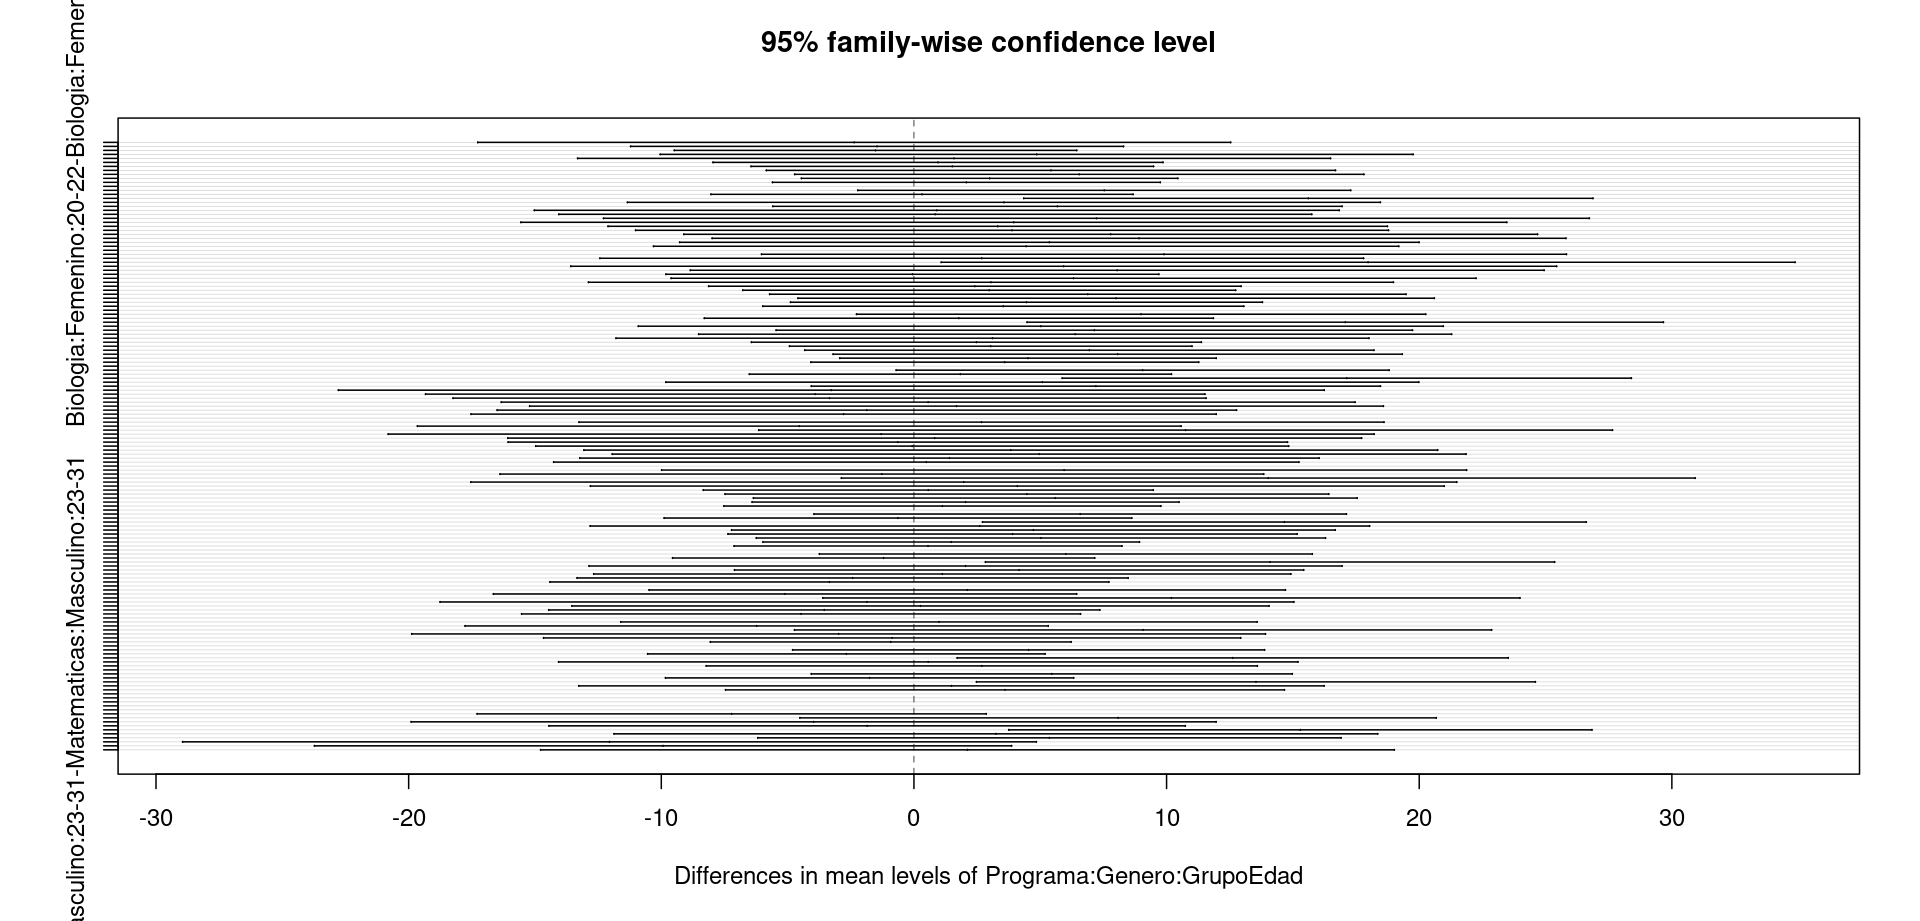
\includegraphics[width=1.0\textwidth]{turkey_Programa-Genero-GrupoEdad.png}
    \caption{Comparaciones múltiples con intervalos de confianza del 95\% para la interacción Programa × Género × GrupoEdad.}
\end{figure}
   
\end{itemize}
\section{Resultados}
\subsection{Verificación de supuestos}

\begin{itemize}
    \item \textbf{Normalidad de los residuos:} Se aplicó la prueba de Shapiro-Wilk, obteniéndose $W = 0.9791$, con un valor $p = 0.3925$. Dado que el valor $p$ es mayor a 0.05, no se rechaza la hipótesis nula de normalidad. Esto indica que los residuos del modelo se distribuyen normalmente.
    
    \item \textbf{Independencia:} Se aplicó la prueba de Durbin-Watson, con un estadístico $DW = 2.2983$ y un valor $p = 0.868$. El valor de $DW$ cercano a 2 sugiere que no existe autocorrelación, y el valor $p$ apoya esta conclusión. Por tanto, se cumple el supuesto de independencia de errores.
    
    \item \textbf{Homogeneidad de varianzas:} Se realizó la prueba de Levene, obteniéndose $F = 1.2476$ con $p = 0.2738$. Como $p > 0.05$, no se rechaza la hipótesis nula de igualdad de varianzas. Por lo tanto, se considera que se cumple la homocedasticidad entre los grupos.

    \item \textbf{ANOVA: }El análisis de varianza indica que el \textbf{grupo de edad} tiene un efecto estadísticamente significativo sobre el IMC (\( p = 0.0001 \)), lo que sugiere que el IMC varía entre los diferentes grupos de edad. En cambio, el \textbf{programa} no presenta diferencias significativas en el IMC (\( p = 0.4876 \)). La variable \textbf{Género} muestra una tendencia cercana a la significancia (\( p = 0.0686 \)), sugiriendo una posible influencia en el IMC.

    Asimismo, se encontraron interacciones significativas entre \textbf{programa y grupo de edad} (\( p = 0.0095 \)), así como en la interacción conjunta de los tres factores (\textbf{programa, género y grupo de edad}) (\( p = 0.0267 \)). Estos resultados indican que el efecto del programa sobre el IMC depende del grupo de edad y de la interacción entre estos factores.
\end{itemize}

\subsection{Comparaciones múltiples}

Se realizó la prueba de Tukey para analizar las diferencias en el índice de masa corporal (IMC) en diferentes niveles de grupo de edad, programa, género y sus combinaciones. A continuación se presentan los hallazgos principales:

\subsubsection{Comparaciones por grupo de edad}

Los resultados indicaron que el grupo de edad de 23--31 años presenta un IMC significativamente mayor en comparación con los grupos de 17--19 años (p = 0.00025) y 20--22 años (p = 0.0233). Sin embargo, no se encontró una diferencia estadísticamente significativa entre los grupos de 20--22 y 17--19 años (p = 0.0821).

\subsubsection{Comparaciones de programa y grupo de edad}

En el análisis de la interacción entre programa y grupo de edad, se observaron varias diferencias significativas (\textit{p} $<$ 0.05). Destacan las siguientes comparaciones:

\begin{itemize}
    \item El programa de Biología en el grupo de 23--31 años tiene un IMC significativamente mayor que en el grupo de 17--19 años (\textit{p} = 0.00009).
    \item Comparaciones entre Biología (23--31 años) y otros programas en el mismo grupo de edad también mostraron diferencias significativas:
    \begin{itemize}
        \item Matemáticas: 23--31 años vs Biología: 17--19 años (\textit{p} = 0.02481)
        \item Biología: 23--31 años vs Matemáticas: 17--19 años (\textit{p} = 0.02210)
        \item Química: 23--31 años vs Biología: 17--19 años (\textit{p} = 0.00123)
    \end{itemize}
    \item Además, se encontraron diferencias entre Biología (23--31 años) y otros grupos de 20--22 años:
    \begin{itemize}
        \item Biología: 23--31 años vs Biología: 20--22 años (\textit{p} = 0.01459)
        \item Biología: 23--31 años vs Matemáticas: 20--22 años (\textit{p} = 0.00237)
        \item Biología: 23--31 años vs Química: 20--22 años (\textit{p} = 0.00331)
    \end{itemize}
\end{itemize}

En general, el grupo de Biología en el rango de 23--31 años mostró un IMC significativamente más alto en comparación con varias combinaciones de programas y grupos de edad más jóvenes, lo cual concuerda con los gráficos de caja realizados.

\subsubsection{Comparaciones entre programas, género y grupo de edad}

El análisis combinado de programa, género y grupo de edad reveló varias diferencias estadísticamente significativas (\textit{p} $<$ 0.05). Algunas comparaciones destacadas incluyen:

\begin{itemize}
    \item La diferencia en IMC entre estudiantes de Matemáticas y Biología, ambos del género femenino en el rango de 17--19 años, fue significativa.
    \item Otras comparaciones entre diferentes combinaciones de programas, género y edad también mostraron diferencias relevantes en los promedios de IMC.
\end{itemize}

Por el contrario, muchas otras comparaciones no alcanzaron significancia estadística (\textit{p} $>$ 0.05), sugiriendo que en esos casos las medias de IMC son similares entre los grupos comparados.
\newpage
\section{Conclusión}

Los resultados del estudio evidencian que el IMC de los estudiantes universitarios varía significativamente según el grupo de edad, y que existen diferencias relevantes cuando se consideran conjuntamente el programa académico, el género y la edad. En particular, el grupo de estudiantes de Biología en el rango de 23 a 31 años presentó un IMC significativamente mayor en comparación con otros subgrupos. Estos hallazgos resaltan la necesidad de diseñar estrategias de promoción de la salud que consideren las características específicas de cada población estudiantil. Entre las recomendaciones derivadas se encuentran: implementar programas de educación nutricional adaptados por edad y programa, fomentar espacios para la actividad física dentro y fuera del entorno académico, promover tamizajes periódicos del estado nutricional, mejorar la oferta alimentaria en la universidad e incorporar la salud y el autocuidado como ejes transversales en la formación integral. Estas acciones permitirían atender de manera más focalizada las necesidades de los estudiantes y contribuir a su bienestar general.
\newpage
\section*{Anexo}


 \newpage
\printbibliography
\end{document}

